\PassOptionsToPackage{unicode=true}{hyperref} % options for packages loaded elsewhere
\PassOptionsToPackage{hyphens}{url}
\PassOptionsToPackage{dvipsnames,svgnames*,x11names*}{xcolor}
%
\documentclass[
  ignorenonframetext,
]{beamer}
\usepackage{pgfpages}
\setbeamertemplate{caption}[numbered]
\setbeamertemplate{caption label separator}{: }
\setbeamercolor{caption name}{fg=normal text.fg}
\beamertemplatenavigationsymbolsempty
% Prevent slide breaks in the middle of a paragraph:
\widowpenalties 1 10000
\raggedbottom
\setbeamertemplate{part page}{
  \centering
  \begin{beamercolorbox}[sep=16pt,center]{part title}
    \usebeamerfont{part title}\insertpart\par
  \end{beamercolorbox}
}
\setbeamertemplate{section page}{
  \centering
  \begin{beamercolorbox}[sep=12pt,center]{part title}
    \usebeamerfont{section title}\insertsection\par
  \end{beamercolorbox}
}
\setbeamertemplate{subsection page}{
  \centering
  \begin{beamercolorbox}[sep=8pt,center]{part title}
    \usebeamerfont{subsection title}\insertsubsection\par
  \end{beamercolorbox}
}
\AtBeginPart{
  \frame{\partpage}
}
\AtBeginSection{
  \ifbibliography
  \else
    \frame{\sectionpage}
  \fi
}
\AtBeginSubsection{
  \frame{\subsectionpage}
}
\usepackage{lmodern}
\usepackage{amssymb,amsmath}
\usepackage{ifxetex,ifluatex}
\ifnum 0\ifxetex 1\fi\ifluatex 1\fi=0 % if pdftex
  \usepackage[T1]{fontenc}
  \usepackage[utf8]{inputenc}
  \usepackage{textcomp} % provides euro and other symbols
\else % if luatex or xelatex
  \usepackage{unicode-math}
  \defaultfontfeatures{Scale=MatchLowercase}
  \defaultfontfeatures[\rmfamily]{Ligatures=TeX,Scale=1}
\fi
% use upquote if available, for straight quotes in verbatim environments
\IfFileExists{upquote.sty}{\usepackage{upquote}}{}
\IfFileExists{microtype.sty}{% use microtype if available
  \usepackage[]{microtype}
  \UseMicrotypeSet[protrusion]{basicmath} % disable protrusion for tt fonts
}{}
\makeatletter
\@ifundefined{KOMAClassName}{% if non-KOMA class
  \IfFileExists{parskip.sty}{%
    \usepackage{parskip}
  }{% else
    \setlength{\parindent}{0pt}
    \setlength{\parskip}{6pt plus 2pt minus 1pt}}
}{% if KOMA class
  \KOMAoptions{parskip=half}}
\makeatother
\usepackage{xcolor}
\IfFileExists{xurl.sty}{\usepackage{xurl}}{} % add URL line breaks if available
\IfFileExists{bookmark.sty}{\usepackage{bookmark}}{\usepackage{hyperref}}
\hypersetup{
  pdftitle={Reproducible (and collaborative) science through RStudio},
  pdfauthor={Jenny Rieck \& Derek Beaton},
  colorlinks=true,
  linkcolor=Maroon,
  filecolor=Maroon,
  citecolor=Blue,
  urlcolor=blue,
  breaklinks=true}
\urlstyle{same}  % don't use monospace font for urls
\newif\ifbibliography
\usepackage{color}
\usepackage{fancyvrb}
\newcommand{\VerbBar}{|}
\newcommand{\VERB}{\Verb[commandchars=\\\{\}]}
\DefineVerbatimEnvironment{Highlighting}{Verbatim}{commandchars=\\\{\}}
% Add ',fontsize=\small' for more characters per line
\usepackage{framed}
\definecolor{shadecolor}{RGB}{248,248,248}
\newenvironment{Shaded}{\begin{snugshade}}{\end{snugshade}}
\newcommand{\AlertTok}[1]{\textcolor[rgb]{0.94,0.16,0.16}{#1}}
\newcommand{\AnnotationTok}[1]{\textcolor[rgb]{0.56,0.35,0.01}{\textbf{\textit{#1}}}}
\newcommand{\AttributeTok}[1]{\textcolor[rgb]{0.77,0.63,0.00}{#1}}
\newcommand{\BaseNTok}[1]{\textcolor[rgb]{0.00,0.00,0.81}{#1}}
\newcommand{\BuiltInTok}[1]{#1}
\newcommand{\CharTok}[1]{\textcolor[rgb]{0.31,0.60,0.02}{#1}}
\newcommand{\CommentTok}[1]{\textcolor[rgb]{0.56,0.35,0.01}{\textit{#1}}}
\newcommand{\CommentVarTok}[1]{\textcolor[rgb]{0.56,0.35,0.01}{\textbf{\textit{#1}}}}
\newcommand{\ConstantTok}[1]{\textcolor[rgb]{0.00,0.00,0.00}{#1}}
\newcommand{\ControlFlowTok}[1]{\textcolor[rgb]{0.13,0.29,0.53}{\textbf{#1}}}
\newcommand{\DataTypeTok}[1]{\textcolor[rgb]{0.13,0.29,0.53}{#1}}
\newcommand{\DecValTok}[1]{\textcolor[rgb]{0.00,0.00,0.81}{#1}}
\newcommand{\DocumentationTok}[1]{\textcolor[rgb]{0.56,0.35,0.01}{\textbf{\textit{#1}}}}
\newcommand{\ErrorTok}[1]{\textcolor[rgb]{0.64,0.00,0.00}{\textbf{#1}}}
\newcommand{\ExtensionTok}[1]{#1}
\newcommand{\FloatTok}[1]{\textcolor[rgb]{0.00,0.00,0.81}{#1}}
\newcommand{\FunctionTok}[1]{\textcolor[rgb]{0.00,0.00,0.00}{#1}}
\newcommand{\ImportTok}[1]{#1}
\newcommand{\InformationTok}[1]{\textcolor[rgb]{0.56,0.35,0.01}{\textbf{\textit{#1}}}}
\newcommand{\KeywordTok}[1]{\textcolor[rgb]{0.13,0.29,0.53}{\textbf{#1}}}
\newcommand{\NormalTok}[1]{#1}
\newcommand{\OperatorTok}[1]{\textcolor[rgb]{0.81,0.36,0.00}{\textbf{#1}}}
\newcommand{\OtherTok}[1]{\textcolor[rgb]{0.56,0.35,0.01}{#1}}
\newcommand{\PreprocessorTok}[1]{\textcolor[rgb]{0.56,0.35,0.01}{\textit{#1}}}
\newcommand{\RegionMarkerTok}[1]{#1}
\newcommand{\SpecialCharTok}[1]{\textcolor[rgb]{0.00,0.00,0.00}{#1}}
\newcommand{\SpecialStringTok}[1]{\textcolor[rgb]{0.31,0.60,0.02}{#1}}
\newcommand{\StringTok}[1]{\textcolor[rgb]{0.31,0.60,0.02}{#1}}
\newcommand{\VariableTok}[1]{\textcolor[rgb]{0.00,0.00,0.00}{#1}}
\newcommand{\VerbatimStringTok}[1]{\textcolor[rgb]{0.31,0.60,0.02}{#1}}
\newcommand{\WarningTok}[1]{\textcolor[rgb]{0.56,0.35,0.01}{\textbf{\textit{#1}}}}
\usepackage{graphicx,grffile}
\makeatletter
\def\maxwidth{\ifdim\Gin@nat@width>\linewidth\linewidth\else\Gin@nat@width\fi}
\def\maxheight{\ifdim\Gin@nat@height>\textheight\textheight\else\Gin@nat@height\fi}
\makeatother
% Scale images if necessary, so that they will not overflow the page
% margins by default, and it is still possible to overwrite the defaults
% using explicit options in \includegraphics[width, height, ...]{}
\setkeys{Gin}{width=\maxwidth,height=\maxheight,keepaspectratio}
\setlength{\emergencystretch}{3em}  % prevent overfull lines
\providecommand{\tightlist}{%
  \setlength{\itemsep}{0pt}\setlength{\parskip}{0pt}}
\setcounter{secnumdepth}{-2}

% set default figure placement to htbp
\makeatletter
\def\fps@figure{htbp}
\makeatother


\title{Reproducible (and collaborative) science through RStudio}
\subtitle{A whirlwind tour with R, RMarkdown, Python, LaTeX, and more}
\author{Jenny Rieck \& Derek Beaton}
\date{May 20 2019}

\begin{document}
\frame{\titlepage}

\begin{frame}{The big outline}
\protect\hypertarget{the-big-outline}{}

\begin{itemize}
\tightlist
\item
  Part 0: Background
\item
  Part 1: A bit about R
\item
  Part 2: RStudio \& Project setup
\item
  Part 3: R, RMarkdown, \& more
\item
  Part 4: Advanced, beyond, \& our favorites
\end{itemize}

\end{frame}

\hypertarget{part-0-background}{%
\section{Part 0: Background}\label{part-0-background}}

\begin{frame}{To dive right in}
\protect\hypertarget{to-dive-right-in}{}

If you want to skip over the background \& RStudio, go straight to
\protect\hyperlink{part-2-rstudio-project-setup}{Part 2: RStudio \&
Project setup}

\end{frame}

\begin{frame}[fragile]{Background}
\protect\hypertarget{background}{}

\begin{itemize}
\tightlist
\item
  This is a taste and to bring you into a bigger world

  \begin{itemize}
  \tightlist
  \item
    R, Python, SQL, and JavaScript are critical data science
    tools/languages
  \end{itemize}
\item
  R (language and community) strongly emphasizes

  \begin{itemize}
  \tightlist
  \item
    Centralization \& standards
  \item
    Rigor \& reproducibility (packages, RMarkdown)
  \end{itemize}
\item
  An interesting language

  \begin{itemize}
  \tightlist
  \item
    Functional
  \item
    With a sublanguage (or dialect?): the \texttt{tidyverse}
  \end{itemize}
\end{itemize}

\end{frame}

\begin{frame}{R is a community (actually many communities!)}
\protect\hypertarget{r-is-a-community-actually-many-communities}{}

\begin{itemize}
\tightlist
\item
  Help and resources
\item
  Package development and distribution
\item
  An ideal example

  \begin{itemize}
  \tightlist
  \item
    Not quite always that way
  \item
    Strong communal presence
  \end{itemize}
\end{itemize}

\end{frame}

\begin{frame}{R: Help!}
\protect\hypertarget{r-help}{}

\begin{itemize}
\tightlist
\item
  So many websites e.g., \url{https://www.statmethods.net/}
\item
  Online forums (Stack Exchange, r-lists)
\item
  SpringerLink

  \begin{itemize}
  \tightlist
  \item
    All R books for free (pdf format) or for minimal cost (printed)
  \end{itemize}
\item
  Vignettes

  \begin{itemize}
  \tightlist
  \item
    step-by-step instruction guides for packages
  \end{itemize}
\item
  Git

  \begin{itemize}
  \tightlist
  \item
    With open books (via bookdown)
  \end{itemize}
\item
  Twitter \#rstats
\item
  RStudio (website)

  \begin{itemize}
  \tightlist
  \item
    Videos, cheat sheets
  \end{itemize}
\end{itemize}

\end{frame}

\begin{frame}{R Packages}
\protect\hypertarget{r-packages}{}

\begin{itemize}
\tightlist
\item
  Packages are bundles of code made by someone (or many people) for
  everyone to use

  \begin{itemize}
  \tightlist
  \item
    There are packages for everything
  \item
    We'll cover some of the diversity throughout
  \end{itemize}
\item
  Comprehensive \& Reproducible
\item
  Available primarily on CRAN

  \begin{itemize}
  \tightlist
  \item
    But also github (less so: r-forge)
  \end{itemize}
\end{itemize}

\end{frame}

\hypertarget{part-1-a-bit-about-r}{%
\section{Part 1: A bit about R}\label{part-1-a-bit-about-r}}

\begin{frame}{R Background}
\protect\hypertarget{r-background}{}

\begin{itemize}
\tightlist
\item
  Created in 1992 by Gentleman \& Ihaka
\end{itemize}

\emph{{[}we{]} considered the problem of obtaining decent statistical
software for our undergraduate Macintosh lab. After considering the
options, we decided that the most satisfactory alternative was to write
our own. {[}\ldots{}{]} Finally we added some syntactic sugar to make it
look somewhat like S. We call the result ``R''.}

\end{frame}

\begin{frame}{What is R?}
\protect\hypertarget{what-is-r}{}

\begin{itemize}
\tightlist
\item
  R is general purpose programming

  \begin{itemize}
  \tightlist
  \item
    Design around \& for statistics
  \item
    ``for and by statisticians''
  \end{itemize}
\item
  R is a collection of tools

  \begin{itemize}
  \tightlist
  \item
    Pre-packaged software at your disposal
  \end{itemize}
\item
  R is free (as in beer and speech)

  \begin{itemize}
  \tightlist
  \item
    No cost, no restrictions
  \item
    E.g., Microsoft (nee Revolution) R
  \end{itemize}
\item
  R is a functional language

  \begin{itemize}
  \tightlist
  \item
    Turing complete
  \item
    Mathematical functions
  \item
    Pass expressions and functions to and from functions
  \end{itemize}
\end{itemize}

\end{frame}

\begin{frame}[fragile]{R: Data types}
\protect\hypertarget{r-data-types}{}

\begin{itemize}
\tightlist
\item
  Stored as \emph{vectors}

  \begin{itemize}
  \tightlist
  \item
    see \texttt{class()}
  \end{itemize}
\item
  numeric

  \begin{itemize}
  \tightlist
  \item
    real or decimal
  \item
    Includes \texttt{NaN}, \texttt{Inf}, \texttt{-Inf}
  \end{itemize}
\item
  integer
\item
  complex
\item
  character
\item
  logical

  \begin{itemize}
  \tightlist
  \item
    includes \texttt{NA}, \texttt{TRUE}, \texttt{FALSE}
  \end{itemize}
\item
  factor

  \begin{itemize}
  \tightlist
  \item
    factors are usually not your friends
  \item
    generally: stringsAsFactors = F or convert these
  \end{itemize}
\end{itemize}

\end{frame}

\begin{frame}[fragile]{R: factor disasters}
\protect\hypertarget{r-factor-disasters}{}

\begin{Shaded}
\begin{Highlighting}[]
\NormalTok{a_numeric_vector <-}\StringTok{ }\KeywordTok{c}\NormalTok{(}\DecValTok{3}\NormalTok{, }\DecValTok{0}\NormalTok{, }\DecValTok{1}\NormalTok{, }\DecValTok{-2}\NormalTok{, }\DecValTok{2}\NormalTok{, }\DecValTok{5}\NormalTok{, }\DecValTok{5}\NormalTok{, }\DecValTok{2}\NormalTok{, }\DecValTok{1}\NormalTok{)}
\NormalTok{(a_numeric_vector }\OperatorTok{+}\StringTok{ }\DecValTok{1}\NormalTok{)}
\end{Highlighting}
\end{Shaded}

\begin{verbatim}
## [1]  4  1  2 -1  3  6  6  3  2
\end{verbatim}

\begin{Shaded}
\begin{Highlighting}[]
\NormalTok{(a_numeric2factor_vector <-}\StringTok{ }\KeywordTok{as.factor}\NormalTok{(a_numeric_vector))}
\end{Highlighting}
\end{Shaded}

\begin{verbatim}
## [1] 3  0  1  -2 2  5  5  2  1 
## Levels: -2 0 1 2 3 5
\end{verbatim}

\begin{Shaded}
\begin{Highlighting}[]
\NormalTok{(}\KeywordTok{as.numeric}\NormalTok{(a_numeric2factor_vector))}
\end{Highlighting}
\end{Shaded}

\begin{verbatim}
## [1] 5 2 3 1 4 6 6 4 3
\end{verbatim}

\begin{Shaded}
\begin{Highlighting}[]
\NormalTok{(}\KeywordTok{as.numeric}\NormalTok{(}\KeywordTok{as.character}\NormalTok{(a_numeric2factor_vector)))}
\end{Highlighting}
\end{Shaded}

\begin{verbatim}
## [1]  3  0  1 -2  2  5  5  2  1
\end{verbatim}

\end{frame}

\begin{frame}[fragile]{R: Data structures}
\protect\hypertarget{r-data-structures}{}

\begin{itemize}
\tightlist
\item
  Starts counting from 1

  \begin{itemize}
  \tightlist
  \item
    Not 0
  \end{itemize}
\item
  vector{[}1{]}
\item
  matrix{[}1,1{]}
\item
  array{[}1,1,1{]}
\item
  list{[}{[}1{]}{]}

  \begin{itemize}
  \tightlist
  \item
    Can contain mixtures of types
  \item
    or list\$\texttt{name}
  \end{itemize}
\item
  data.frame:

  \begin{itemize}
  \tightlist
  \item
    Is technically a list but access in three ways
  \item
    data.frame{[}{[}1{]}{]}{[}1{]}
  \item
    data.frame{[}1,1{]}
  \item
    data.frame\$\texttt{name}
  \item
    tibbles: tidyverse data.frames
  \end{itemize}
\end{itemize}

\end{frame}

\begin{frame}{R}
\protect\hypertarget{r}{}

Some more about R here\ldots{} Matlab cheat sheet Other cheat sheets

\end{frame}

\begin{frame}{Tidyverse}
\protect\hypertarget{tidyverse}{}

\begin{itemize}
\tightlist
\item
  something here about tidy
\item
  Learn it. But don't learn \emph{only} the tidyverse; you'll be lost in
  base R
\end{itemize}

\end{frame}

\hypertarget{part-2-rstudio-project-setup}{%
\section{Part 2: RStudio \& Project
setup}\label{part-2-rstudio-project-setup}}

\begin{frame}{RStudio}
\protect\hypertarget{rstudio}{}

\begin{itemize}
\tightlist
\item
  IDE: Integrated development environment
\item
  RStudio: Does so much

  \begin{itemize}
  \tightlist
  \item
    We scratch the surface here
  \end{itemize}
\item
  Quick walk through
\item
  Followed by specific set up

  \begin{itemize}
  \tightlist
  \item
    Generally, but
  \item
    Also for this workshop
  \end{itemize}
\end{itemize}

\end{frame}

\begin{frame}{RStudio Environment}
\protect\hypertarget{rstudio-environment}{}

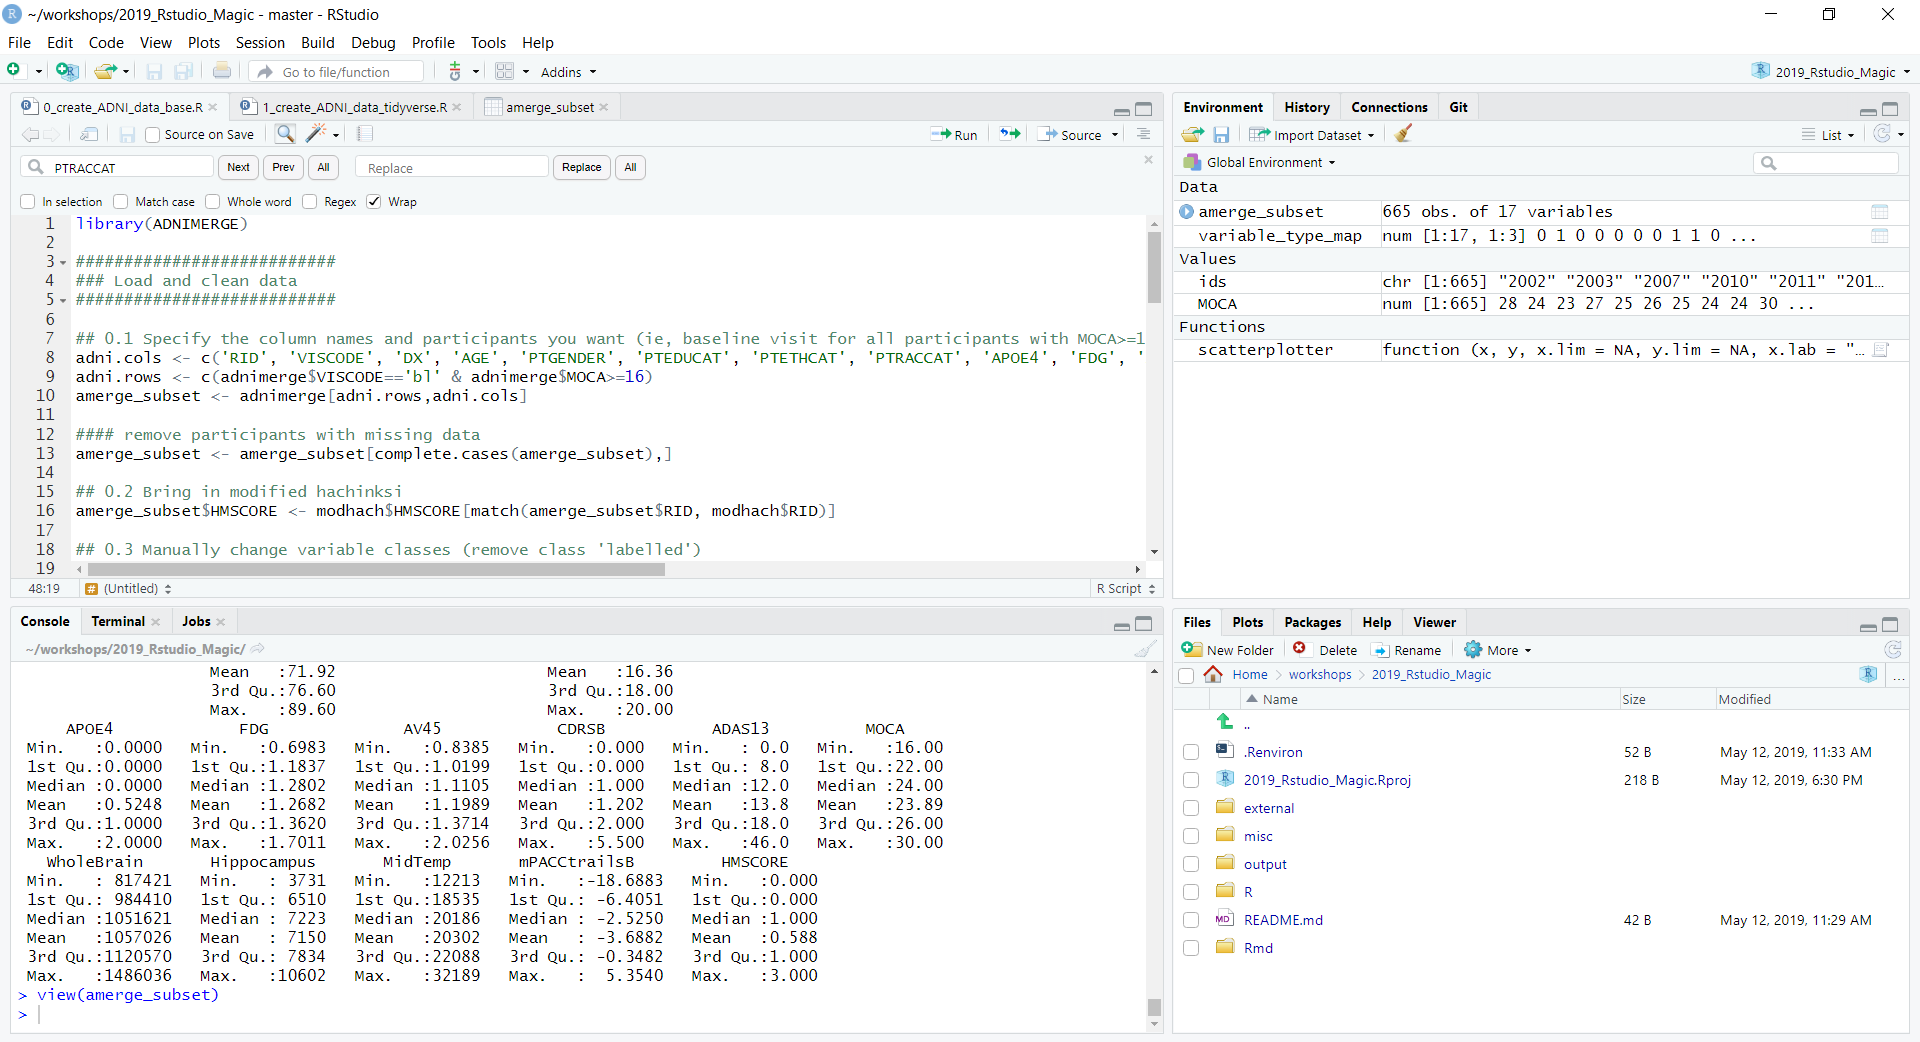
\includegraphics{../external/images/rstudio_0_terminal_code.PNG}

\end{frame}

\begin{frame}{RStudio Environment}
\protect\hypertarget{rstudio-environment-1}{}

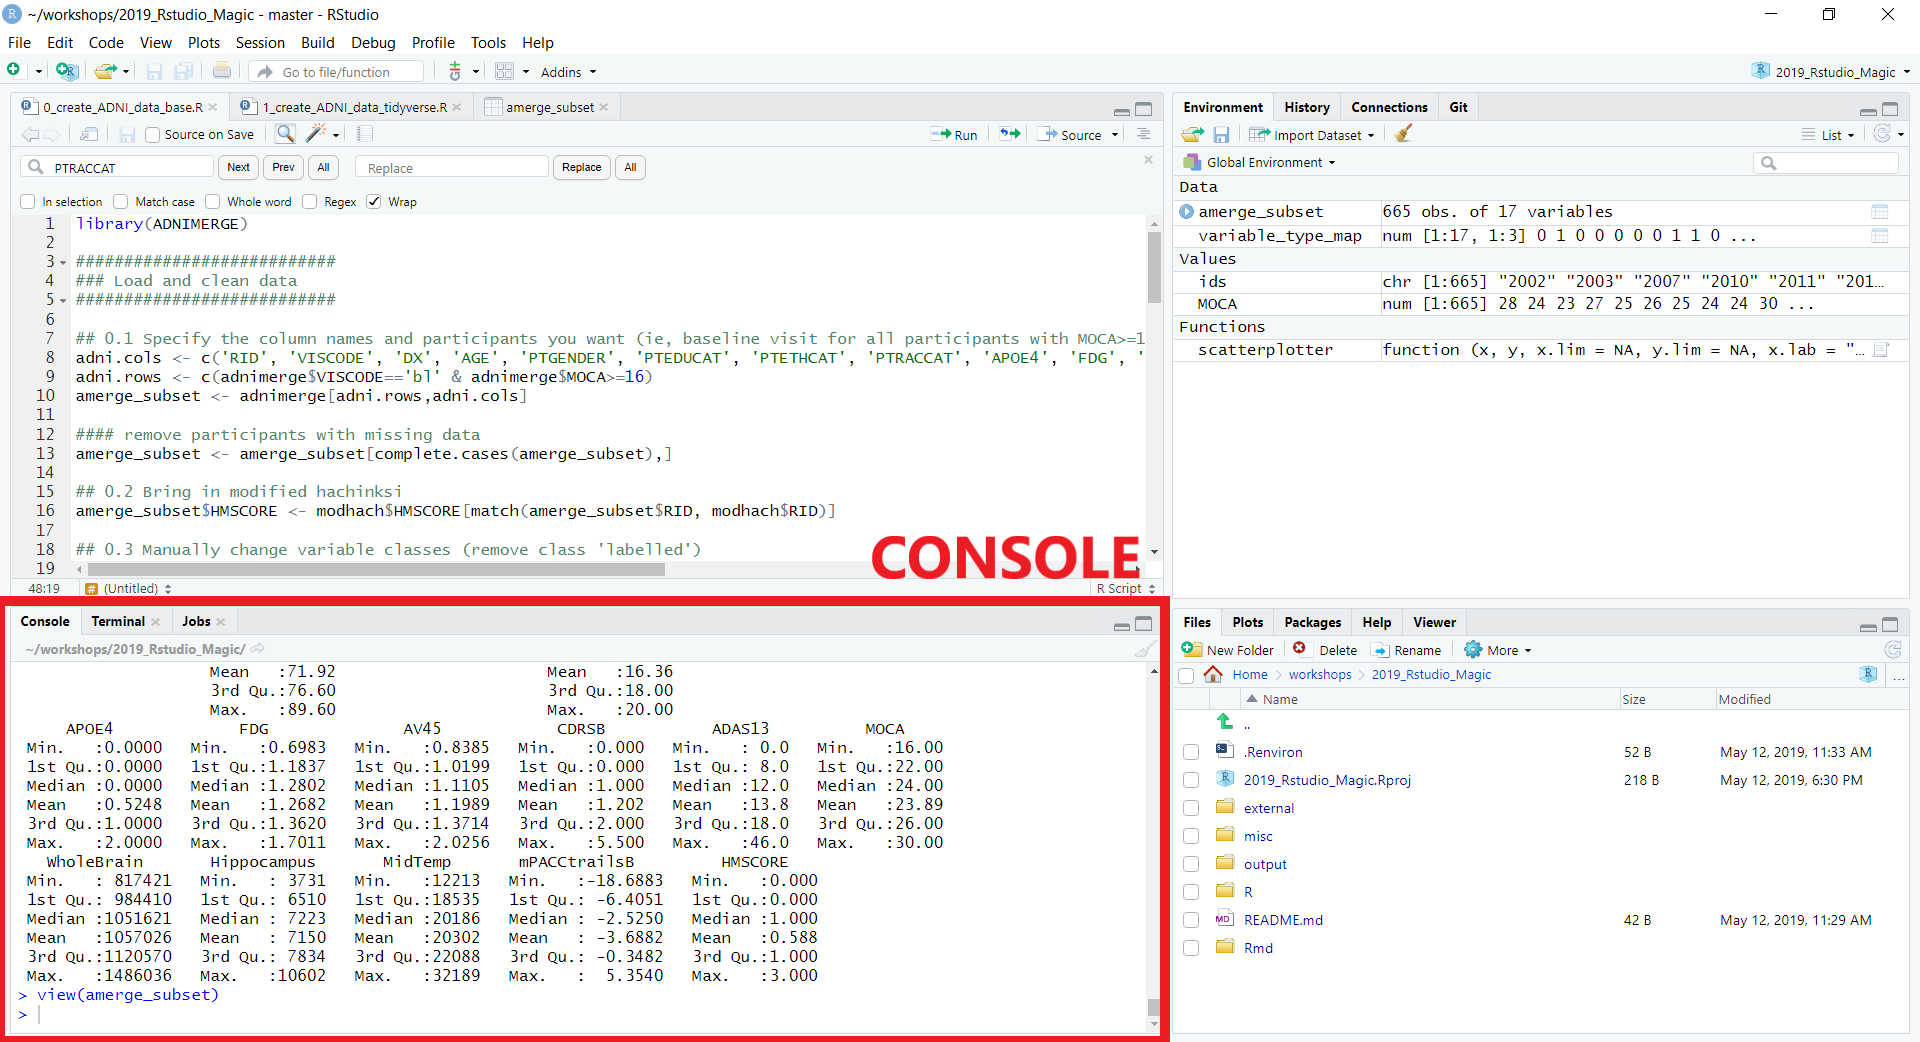
\includegraphics{../external/images/rstudio_terminal_1_CONSOLE.png}

\end{frame}

\begin{frame}{RStudio Environment}
\protect\hypertarget{rstudio-environment-2}{}

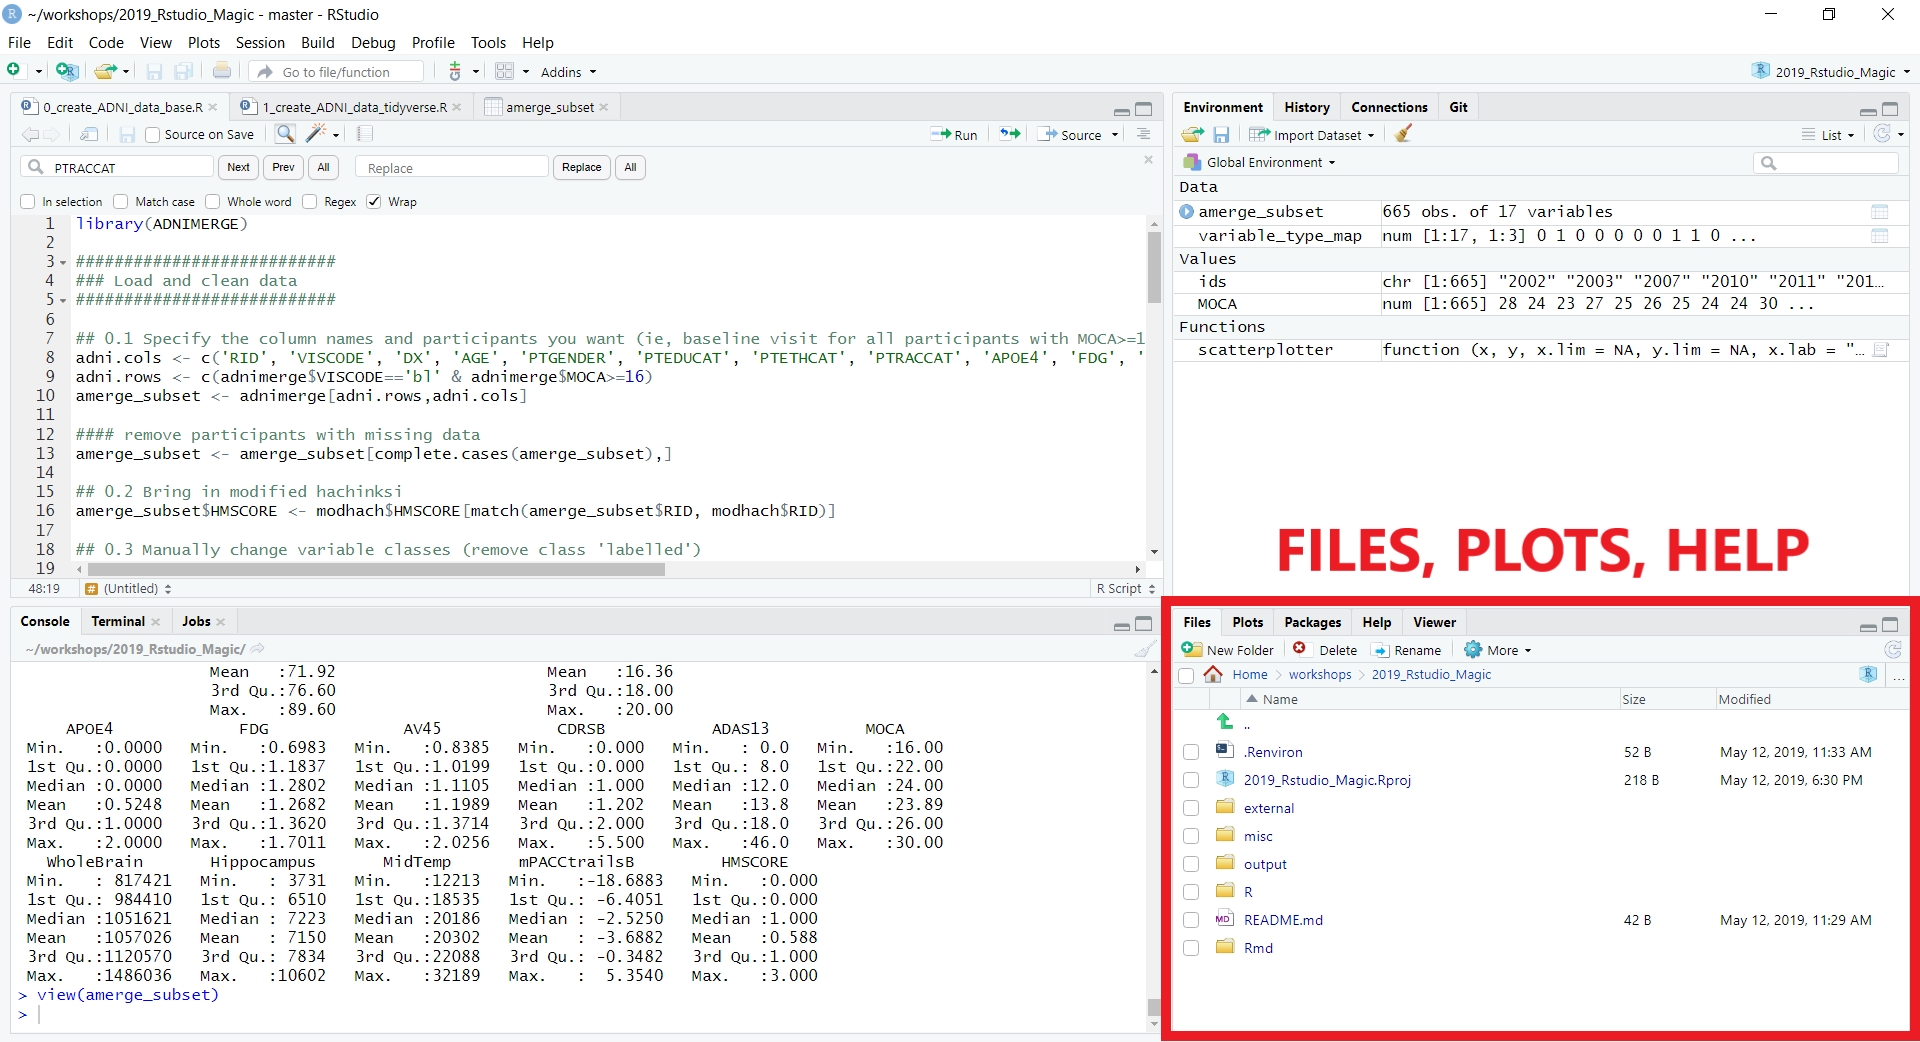
\includegraphics{../external/images/rstudio_terminal_2_FILES.png}

\end{frame}

\begin{frame}{RStudio Environment}
\protect\hypertarget{rstudio-environment-3}{}

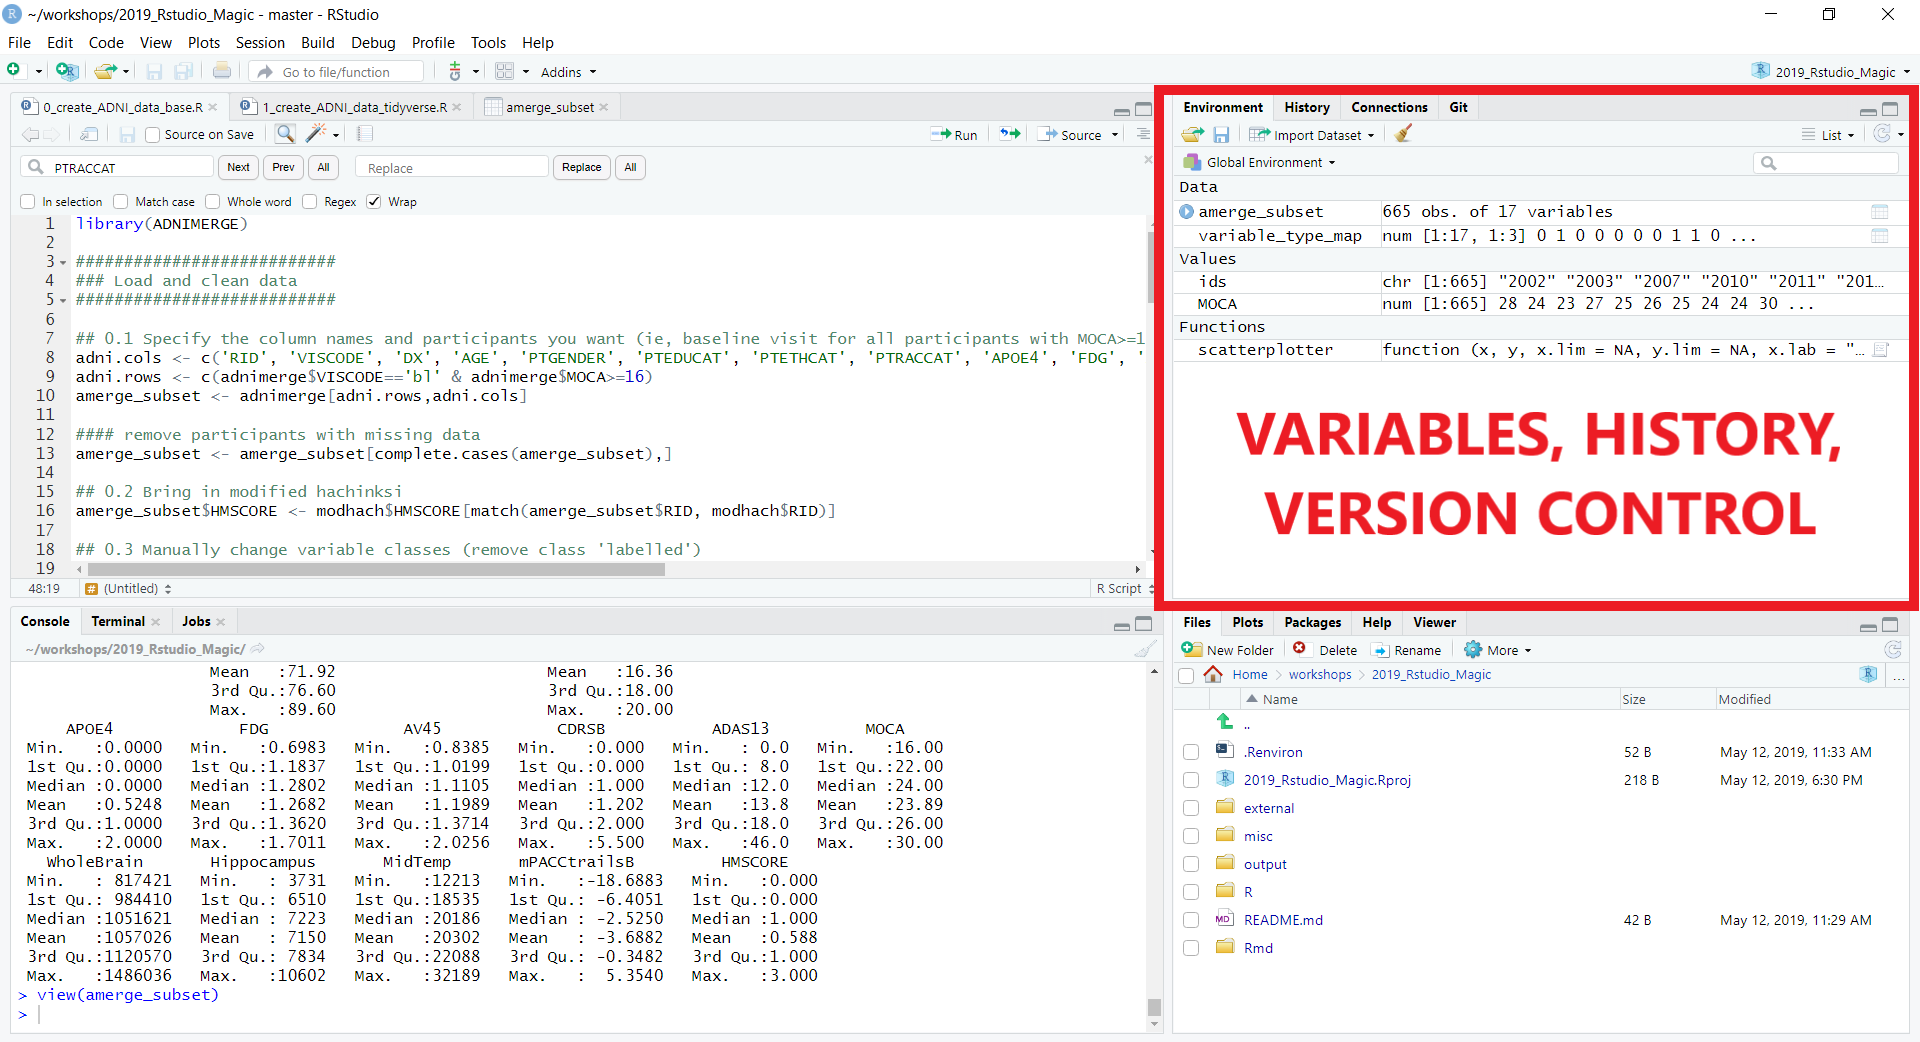
\includegraphics{../external/images/rstudio_terminal_3_ENV.png}

\end{frame}

\begin{frame}{RStudio Environment}
\protect\hypertarget{rstudio-environment-4}{}

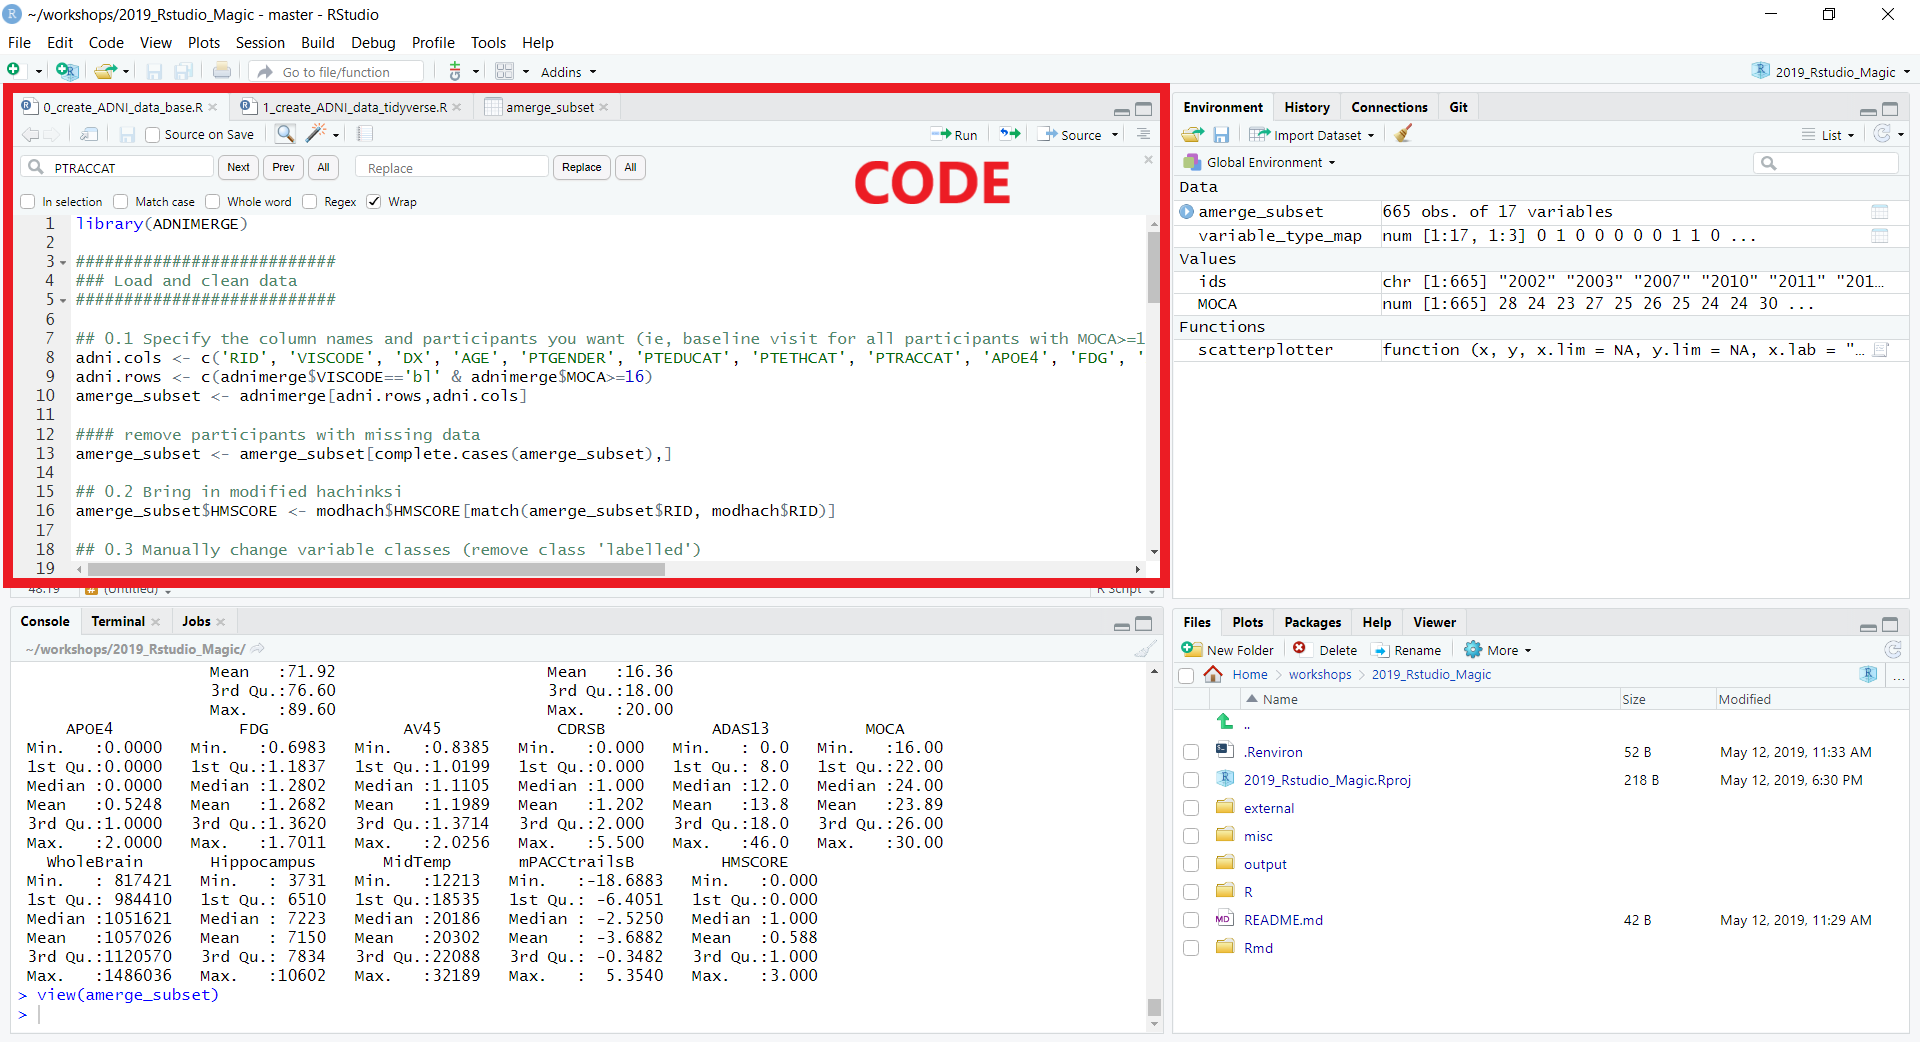
\includegraphics{../external/images/rstudio_terminal_4_CODE.png}

\end{frame}

\begin{frame}{RStudio Environment}
\protect\hypertarget{rstudio-environment-5}{}

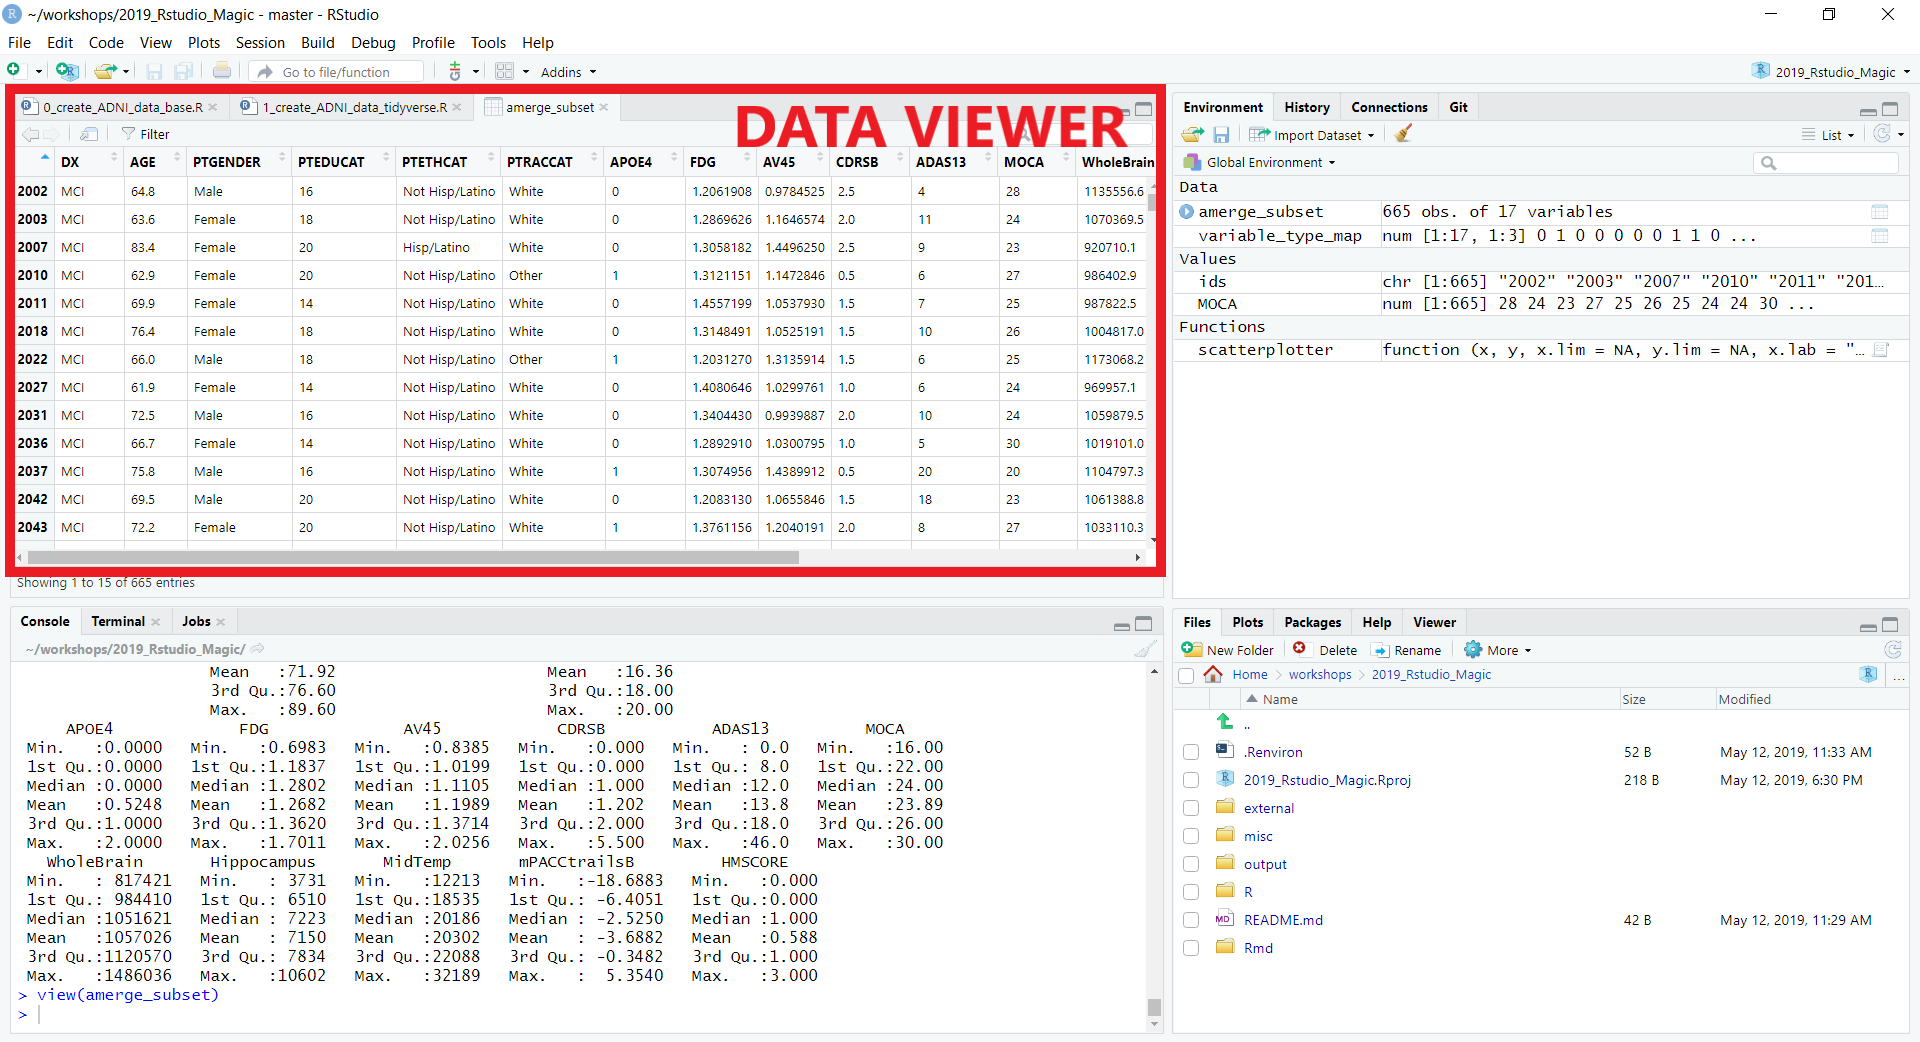
\includegraphics{../external/images/rstudio_terminal_5_DATA.png}

\end{frame}

\begin{frame}{Some benefits of RStudio}
\protect\hypertarget{some-benefits-of-rstudio}{}

\begin{itemize}
\tightlist
\item
  Built-in integration with version control (git or SVN)
\item
  Package and documentation generation
\item
  Reproducible science!

  \begin{itemize}
  \tightlist
  \item
    R Markdown documents

    \begin{itemize}
    \tightlist
    \item
      Save and execute code
    \item
      Generate high quality reports that can be shared
    \end{itemize}
  \item
    Create presentations (like this one!)
  \item
    Even write papers
  \item
    Python, D3 (JavaScript), SQL, Shiny, LaTeX, Git/SVN, HTML/CSS, and
    so much more.
  \end{itemize}
\item
  This workshop

  \begin{itemize}
  \tightlist
  \item
    Will walk you through some of this (and more)
  \item
    See
    \url{https://github.com/jennyrieck/workshops/tree/master/2019_Rstudio_Magic}
  \end{itemize}
\end{itemize}

\end{frame}

\begin{frame}{RStudio is more}
\protect\hypertarget{rstudio-is-more}{}

\begin{itemize}
\tightlist
\item
  Not just an IDE
\item
  A company
\item
  A community
\item
  A conference
\item
  A centralized resource
\end{itemize}

\end{frame}

\begin{frame}{RStudio Resources}
\protect\hypertarget{rstudio-resources}{}

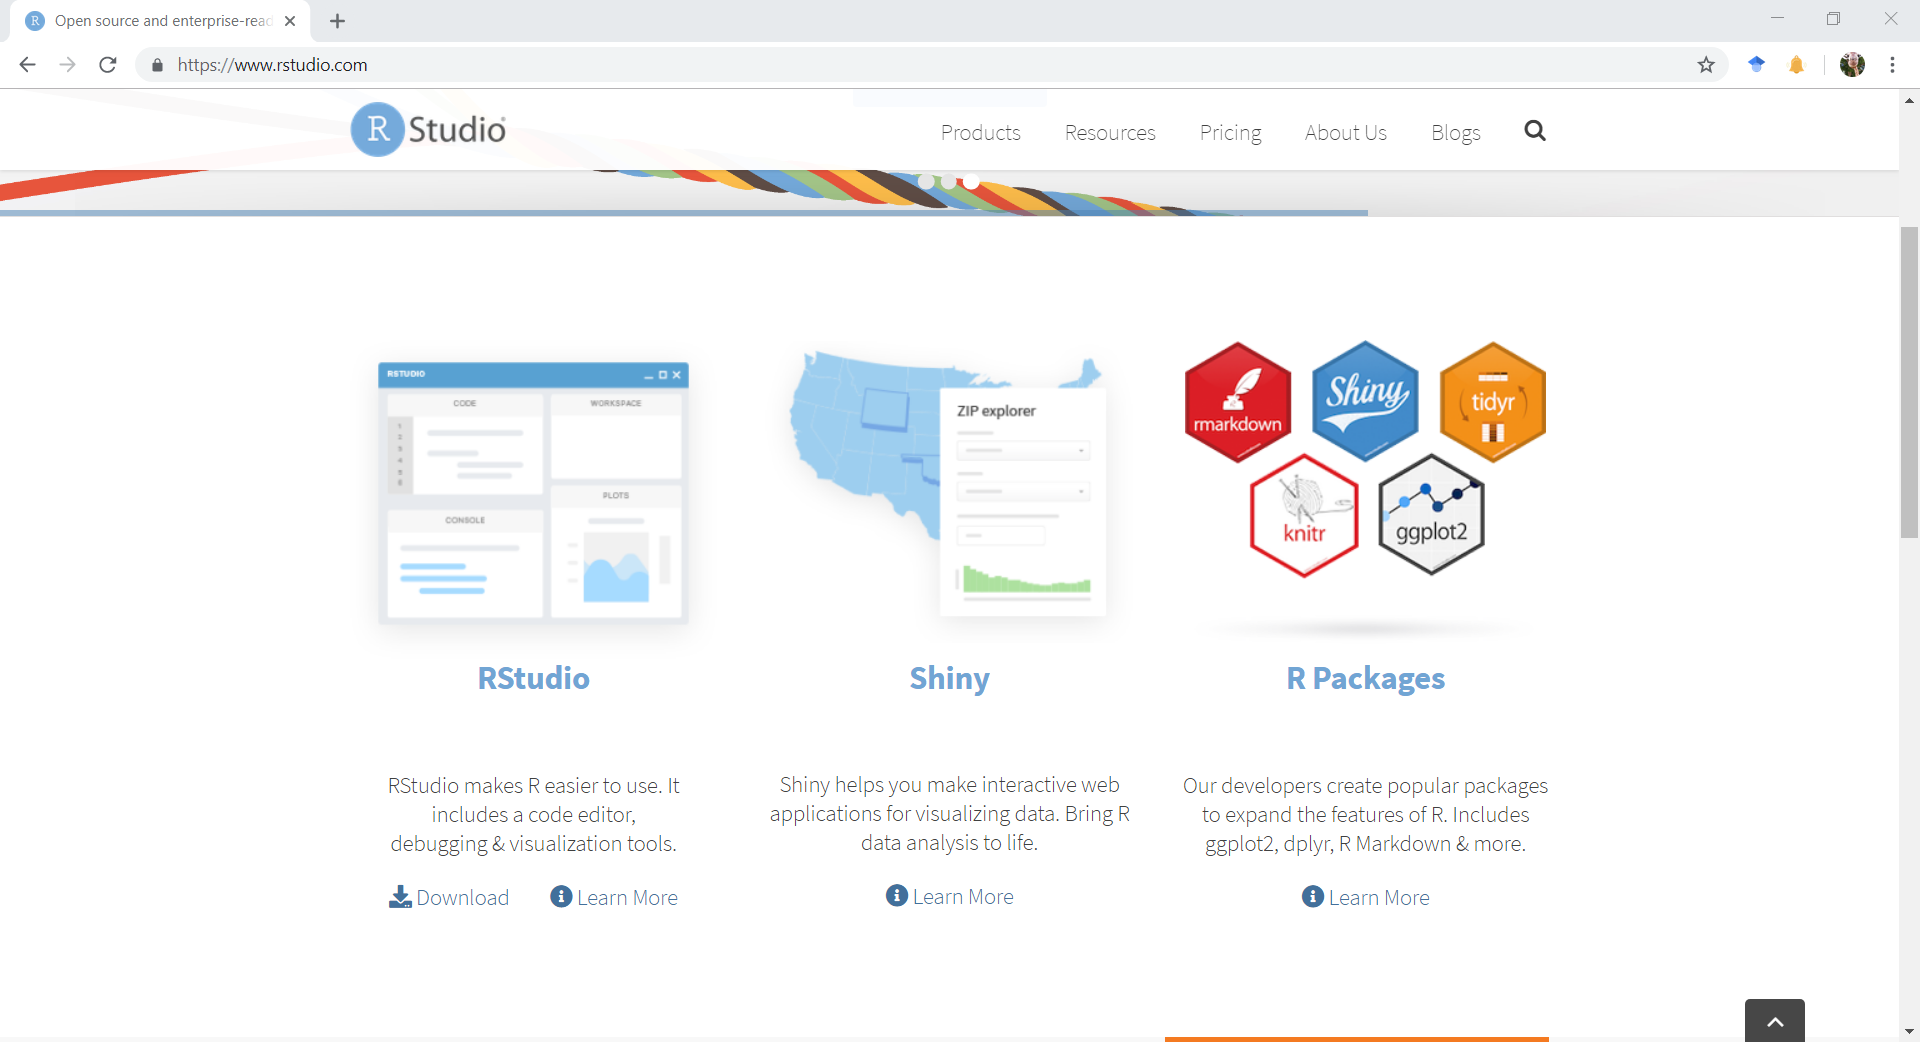
\includegraphics{../external/images/rstudio_dot_com_1_main.PNG}

\end{frame}

\begin{frame}{RStudio Resources}
\protect\hypertarget{rstudio-resources-1}{}

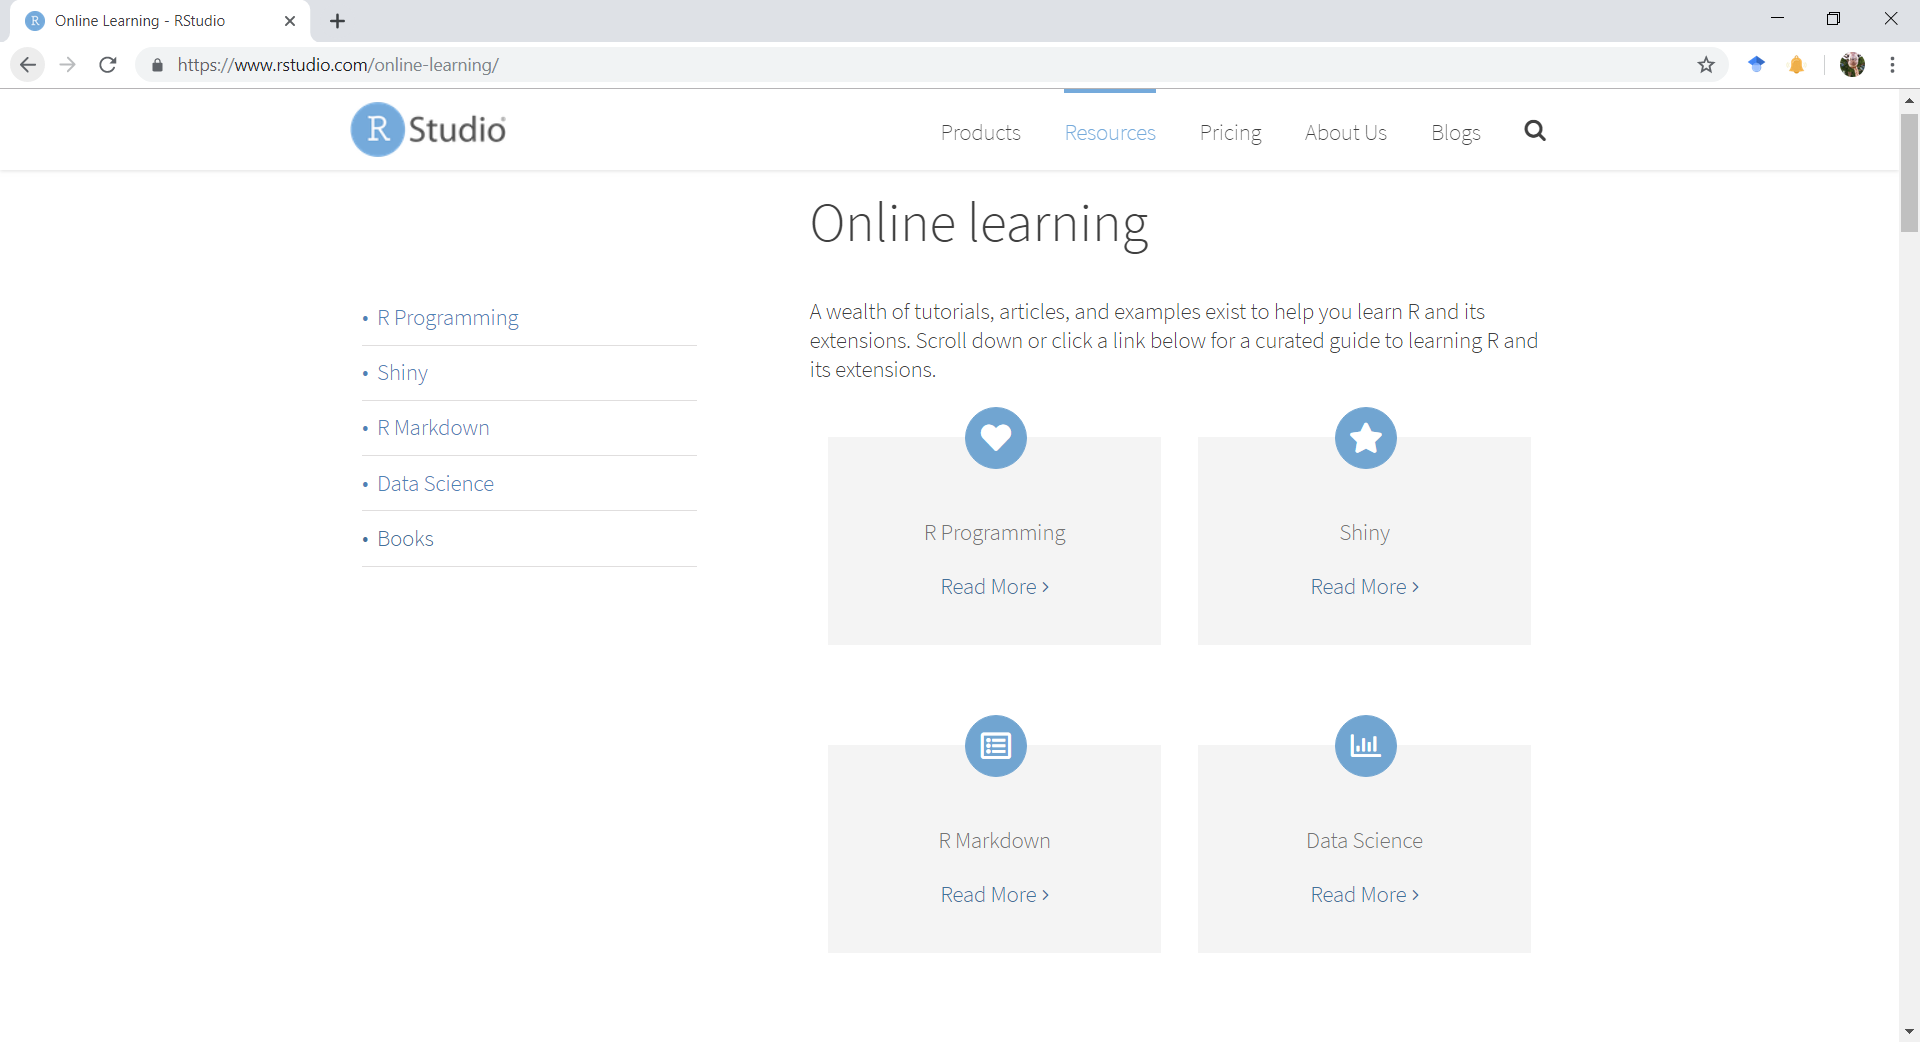
\includegraphics{../external/images/rstudio_dot_com_2_learning.PNG}

\end{frame}

\begin{frame}{RStudio Resources}
\protect\hypertarget{rstudio-resources-2}{}

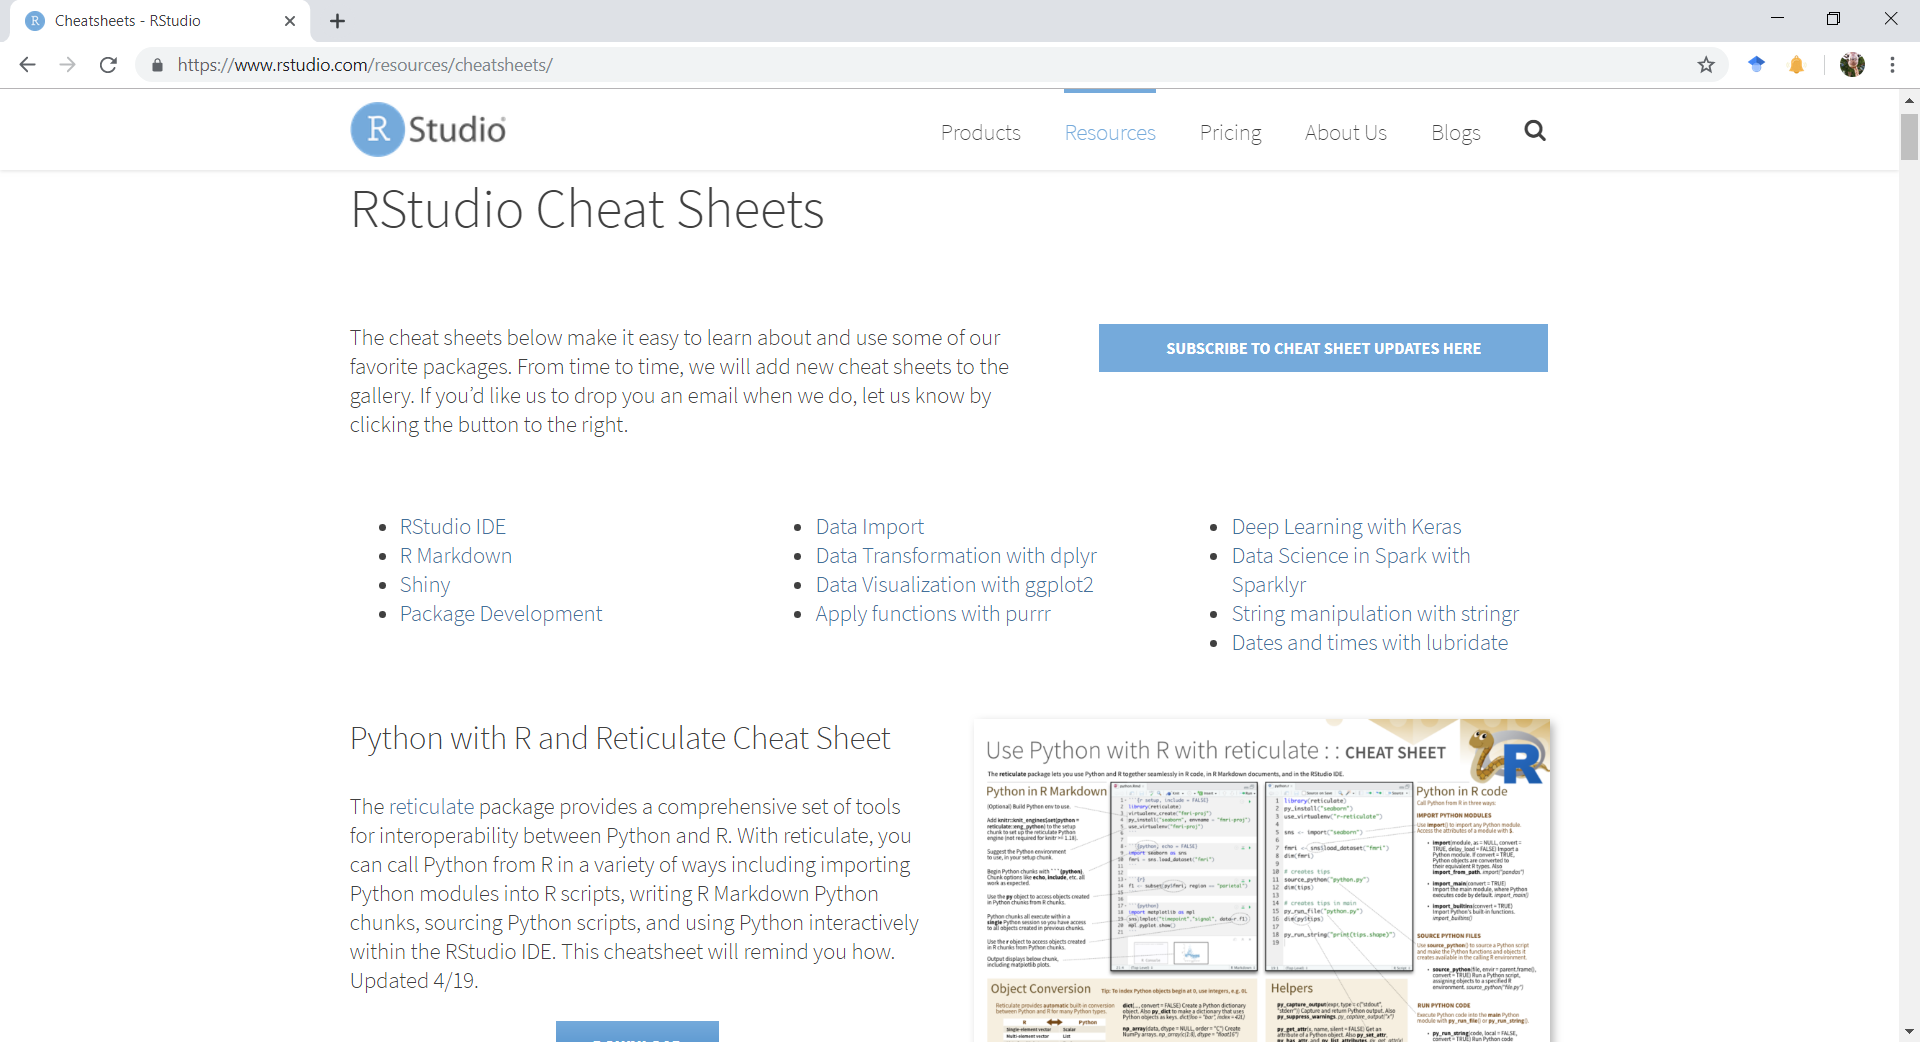
\includegraphics{../external/images/rstudio_dot_com_3_cheats.PNG}

\end{frame}

\begin{frame}{Project and Environment Setup}
\protect\hypertarget{project-and-environment-setup}{}

\begin{itemize}
\tightlist
\item
  Special \& hidden files
\item
  Having a structure
\end{itemize}

\end{frame}

\begin{frame}{RStudio Setup}
\protect\hypertarget{rstudio-setup}{}

\begin{itemize}
\tightlist
\item
  See \url{https://jennybc.github.io/2014-05-12-ubc/r-setup.html} for a
  detailed guide
\end{itemize}

\end{frame}

\begin{frame}{For safety \& collaboration}
\protect\hypertarget{for-safety-collaboration}{}

\begin{itemize}
\tightlist
\item
  Project(s) files

  \begin{itemize}
  \tightlist
  \item
    SOMETHING!
  \end{itemize}
\end{itemize}

\end{frame}

\begin{frame}{Projects through Git}
\protect\hypertarget{projects-through-git}{}

\begin{itemize}
\tightlist
\item
  Create a new project File
  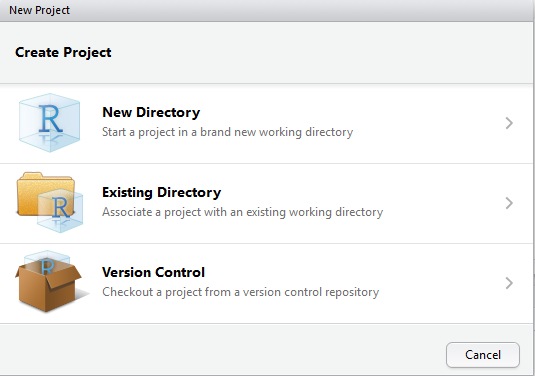
\includegraphics[width=0.75\textwidth,height=\textheight]{../external/images/setup_2_rstudio_project.PNG}
\end{itemize}

\end{frame}

\begin{frame}{Git \& Projects}
\protect\hypertarget{git-projects}{}

\begin{itemize}
\tightlist
\item
  Git

  \begin{itemize}
  \tightlist
  \item
    Download git and link executable within RStudio
    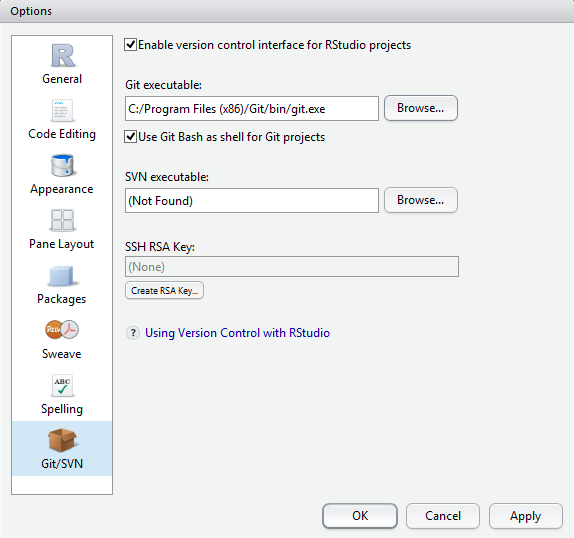
\includegraphics[width=0.6\textwidth,height=\textheight]{../external/images/setup_1_rstudio_git.PNG}
  \end{itemize}
\end{itemize}

\end{frame}

\begin{frame}[fragile]{Format .gitignore}
\protect\hypertarget{format-.gitignore}{}

\begin{itemize}
\tightlist
\item
  File types to ignore via version control

  \begin{itemize}
  \tightlist
  \item
    \texttt{**} before each extentions will match directories anywhere
    in the repo
  \end{itemize}

  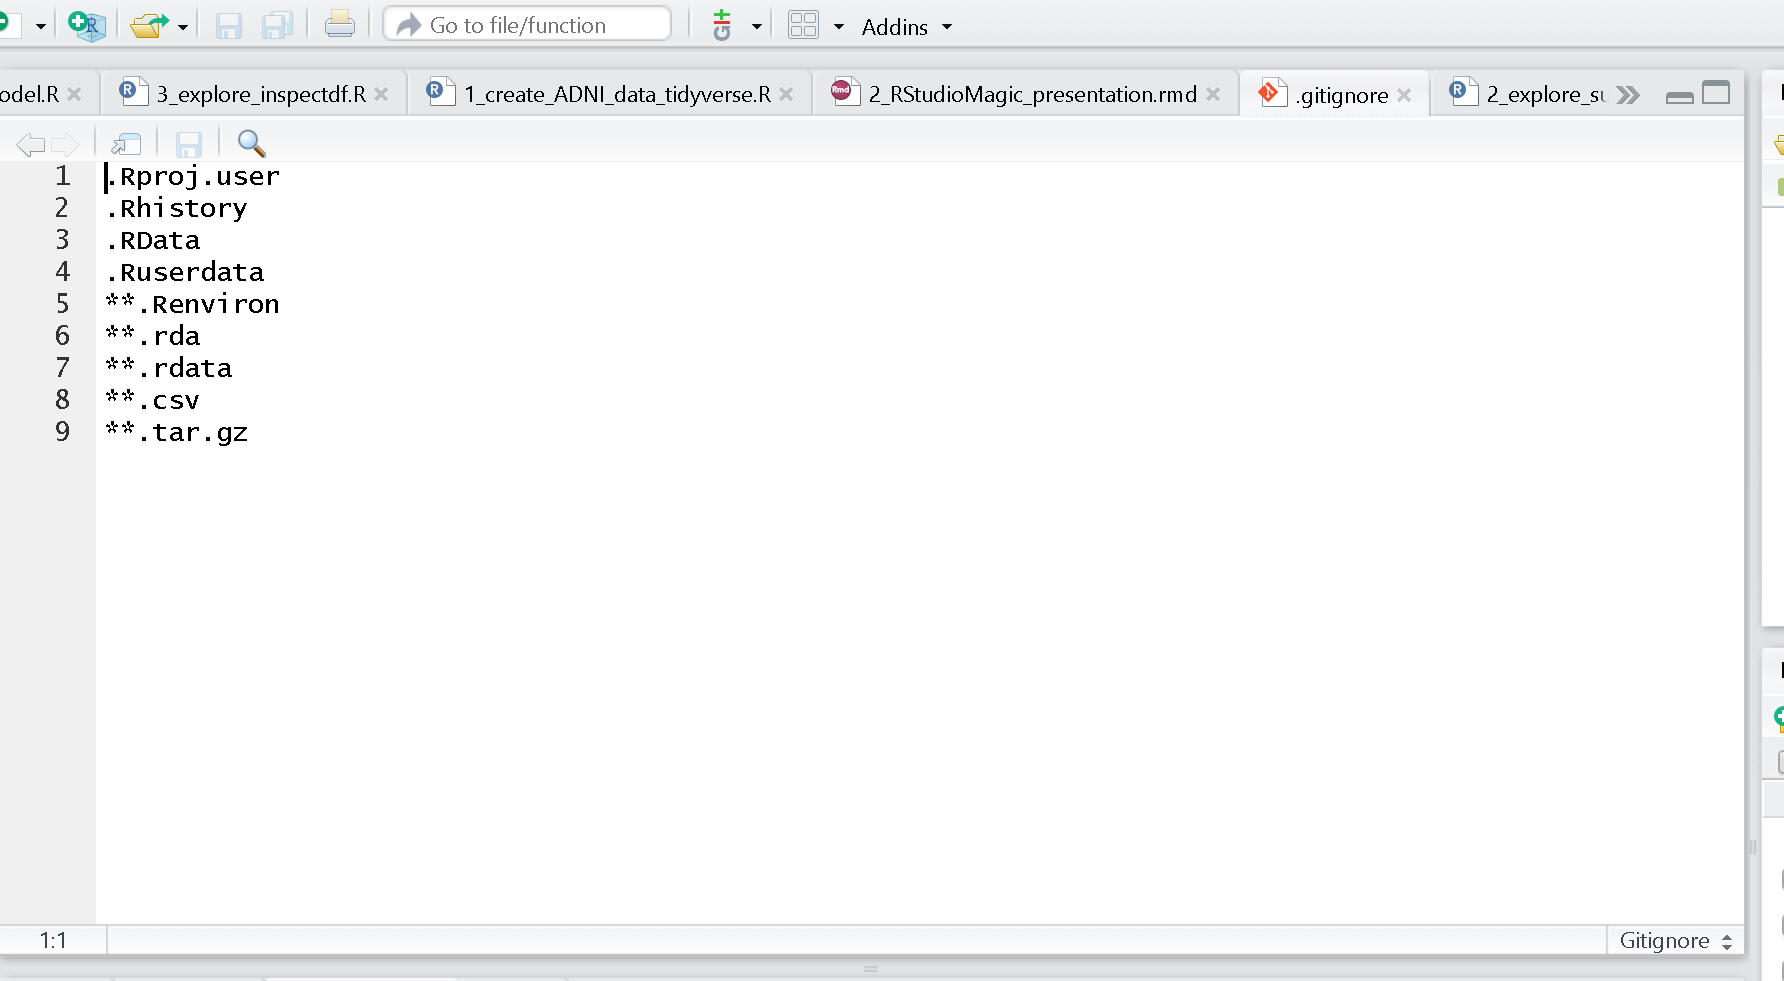
\includegraphics[width=0.75\textwidth,height=\textheight]{../external/images/gitignore.PNG}
\end{itemize}

\end{frame}

\begin{frame}{Environmental variables}
\protect\hypertarget{environmental-variables}{}

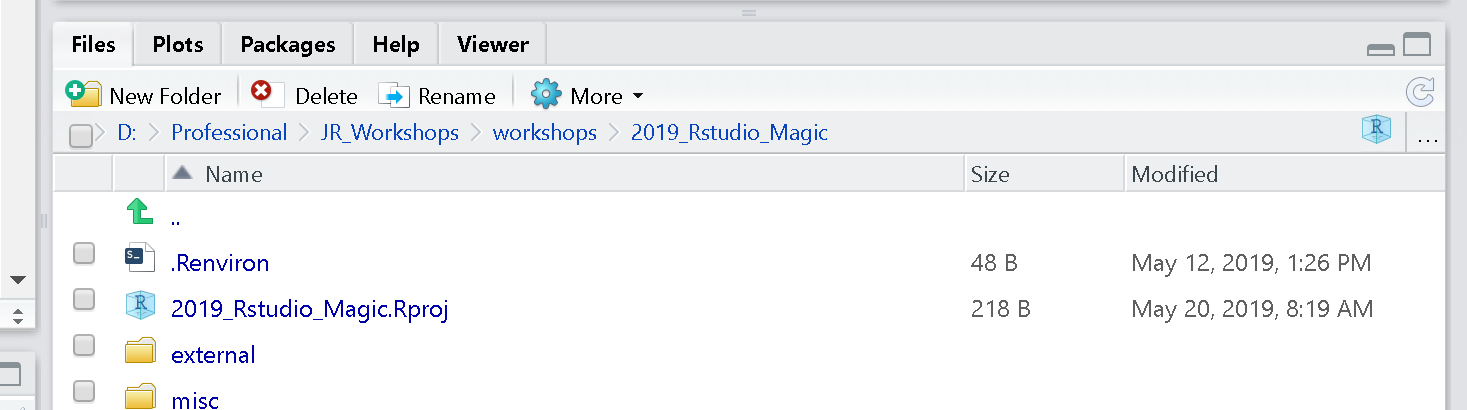
\includegraphics[width=0.6\textwidth,height=\textheight]{../external/images/Revniron.PNG}

\end{frame}

\begin{frame}[fragile]{Format environmental variables}
\protect\hypertarget{format-environmental-variables}{}

\begin{itemize}
\tightlist
\item
  Set environmental variables (ie, directory location of data) to make
  code generalizable across computers

  \begin{itemize}
  \tightlist
  \item
    Don't commit or share these
  \end{itemize}
\item
  In \textbf{your} project folder create a \texttt{.Renviron} file and
  define variables

  \begin{itemize}
  \tightlist
  \item
    Jenny's:
  \end{itemize}

  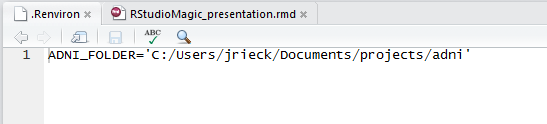
\includegraphics[width=0.6\textwidth,height=\textheight]{../external/images/setup_3_rstudio_project_environ.PNG}

  \begin{itemize}
  \tightlist
  \item
    Derek's:
  \end{itemize}

  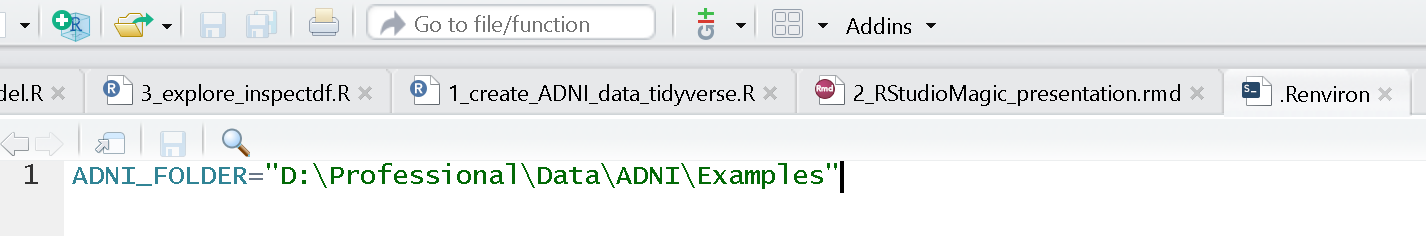
\includegraphics[width=0.8\textwidth,height=\textheight]{../external/images/setup_3_rstudio_project_environ2.PNG}
\end{itemize}

\end{frame}

\begin{frame}{Organize your project folders and markdown}
\protect\hypertarget{organize-your-project-folders-and-markdown}{}

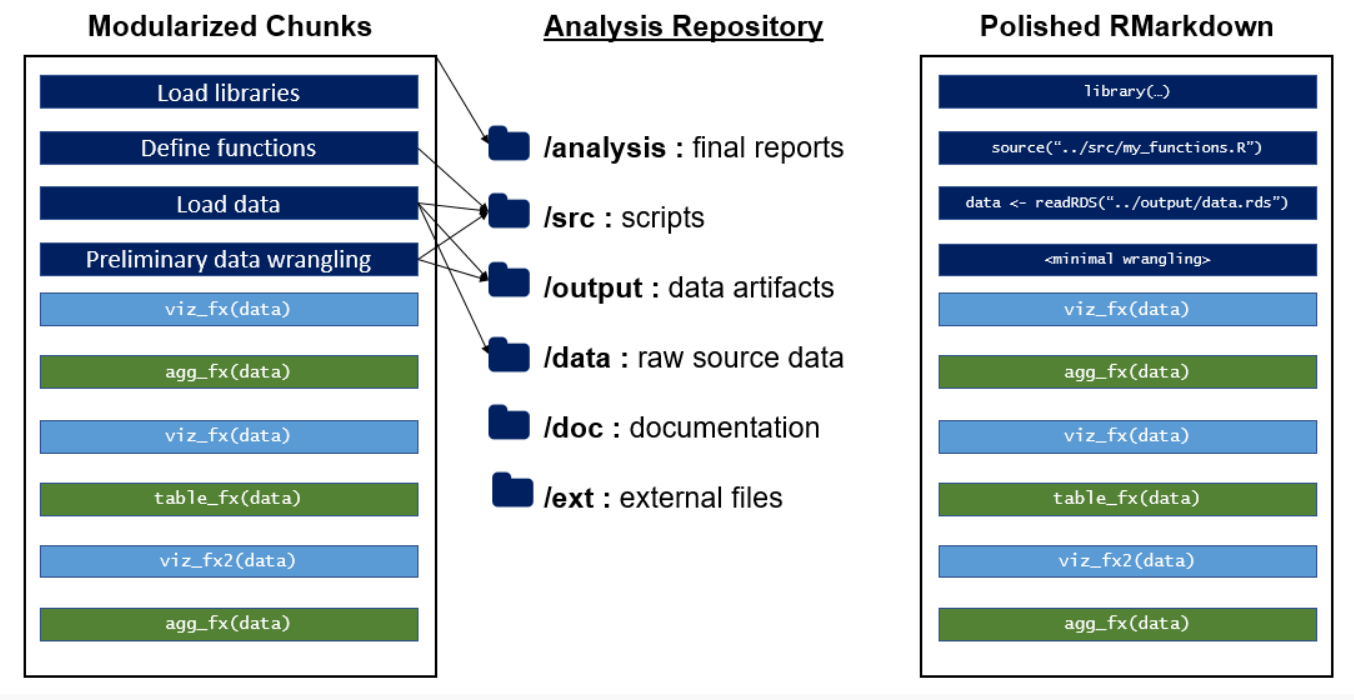
\includegraphics{../external/images/setup_4_markdown_project.PNG}

\url{https://emilyriederer.netlify.com/post/rmarkdown-driven-development/}

\end{frame}

\begin{frame}{Organize your project folders and markdown}
\protect\hypertarget{organize-your-project-folders-and-markdown-1}{}

\begin{itemize}
\tightlist
\item
  What works for you?
\item
  What works for your organization or team?
\item
  Maximize utility, minimize complexity
\end{itemize}

\end{frame}

\begin{frame}{This works for us}
\protect\hypertarget{this-works-for-us}{}

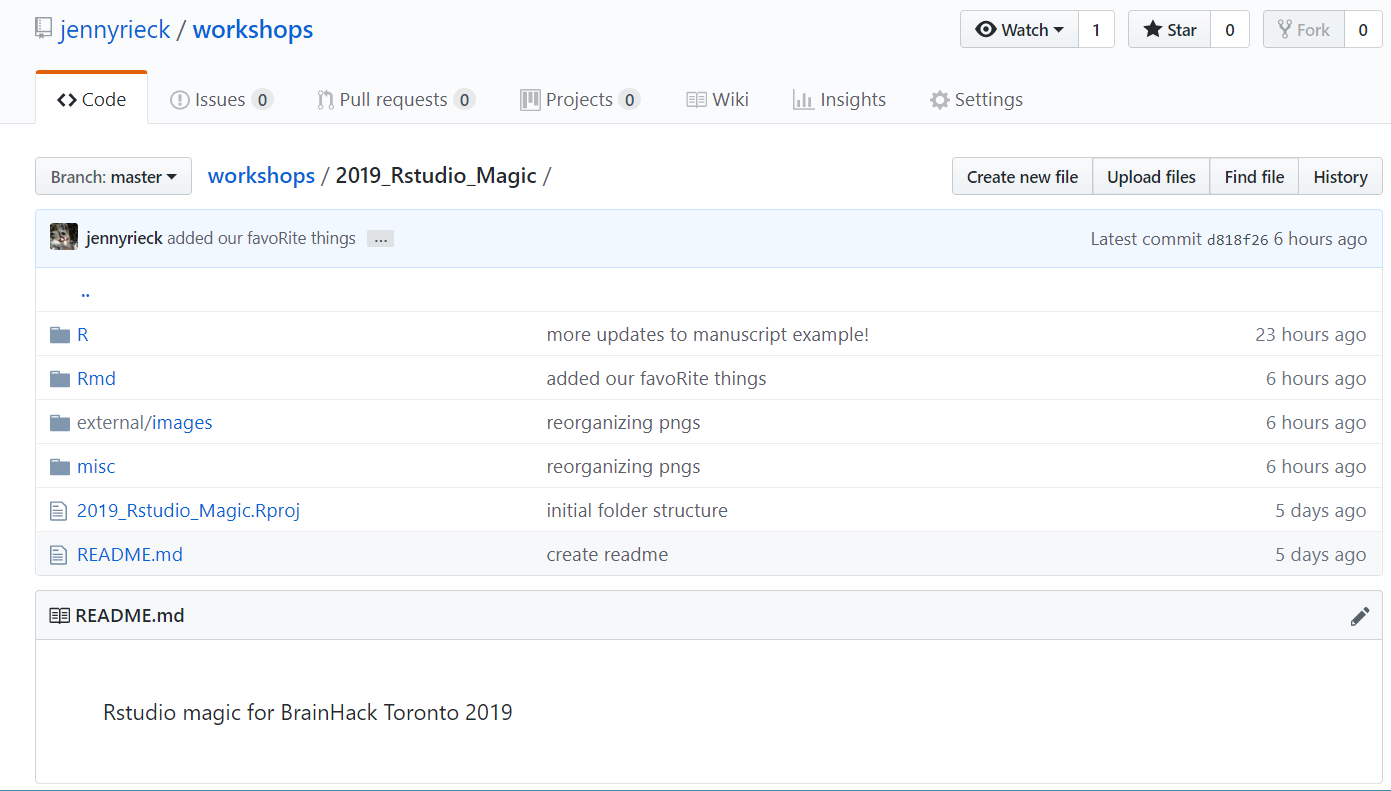
\includegraphics{../external/images/setup_5_git.PNG}

\end{frame}

\begin{frame}{This works for us}
\protect\hypertarget{this-works-for-us-1}{}

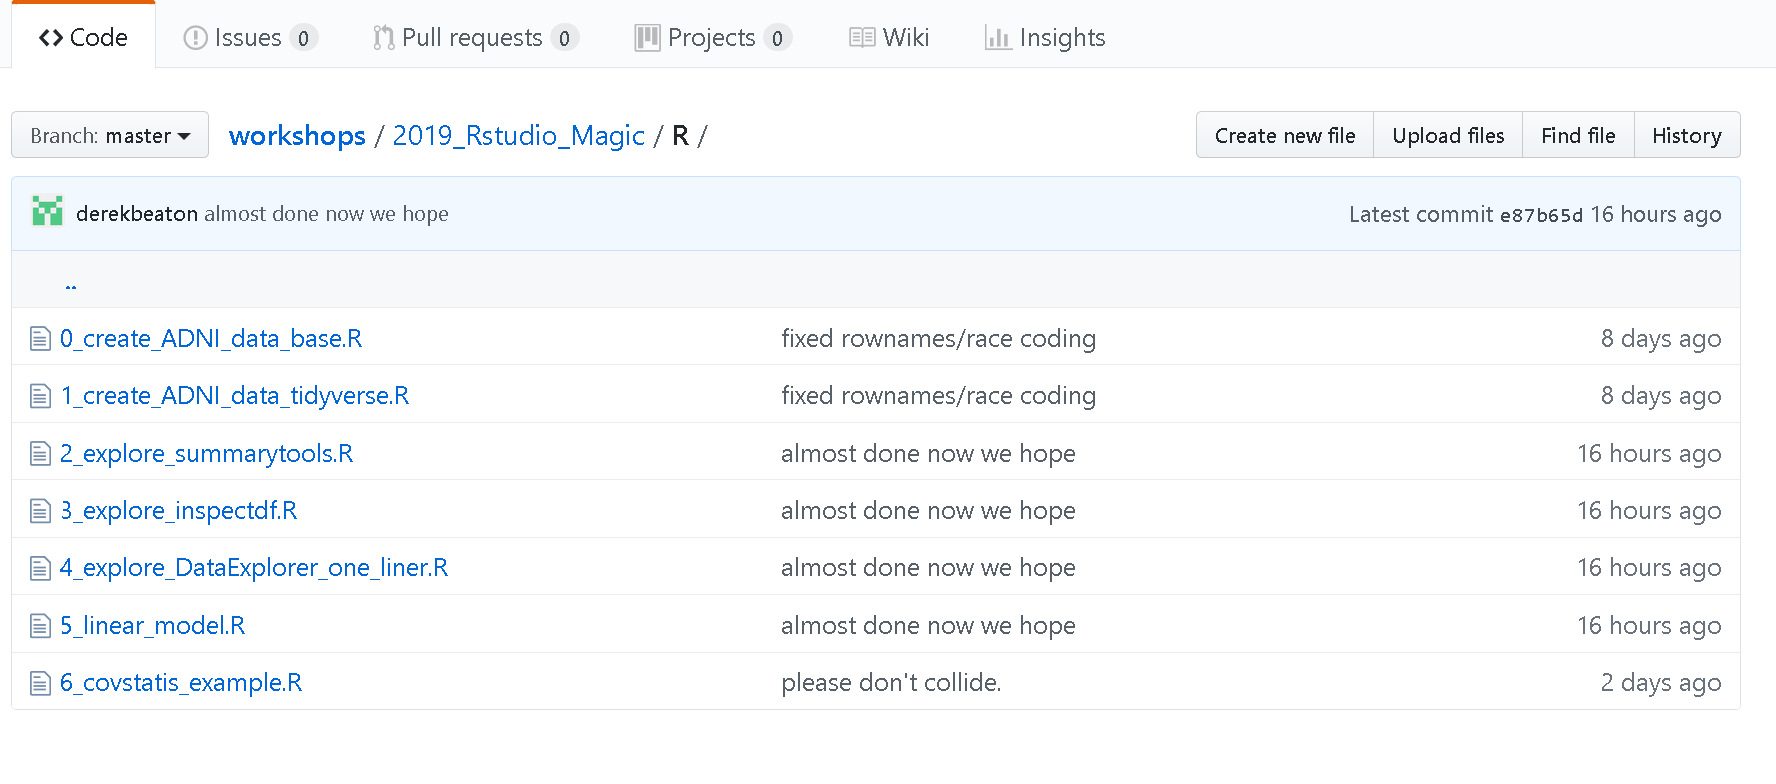
\includegraphics{../external/images/Rfolder.PNG}

\end{frame}

\begin{frame}{This works for us}
\protect\hypertarget{this-works-for-us-2}{}

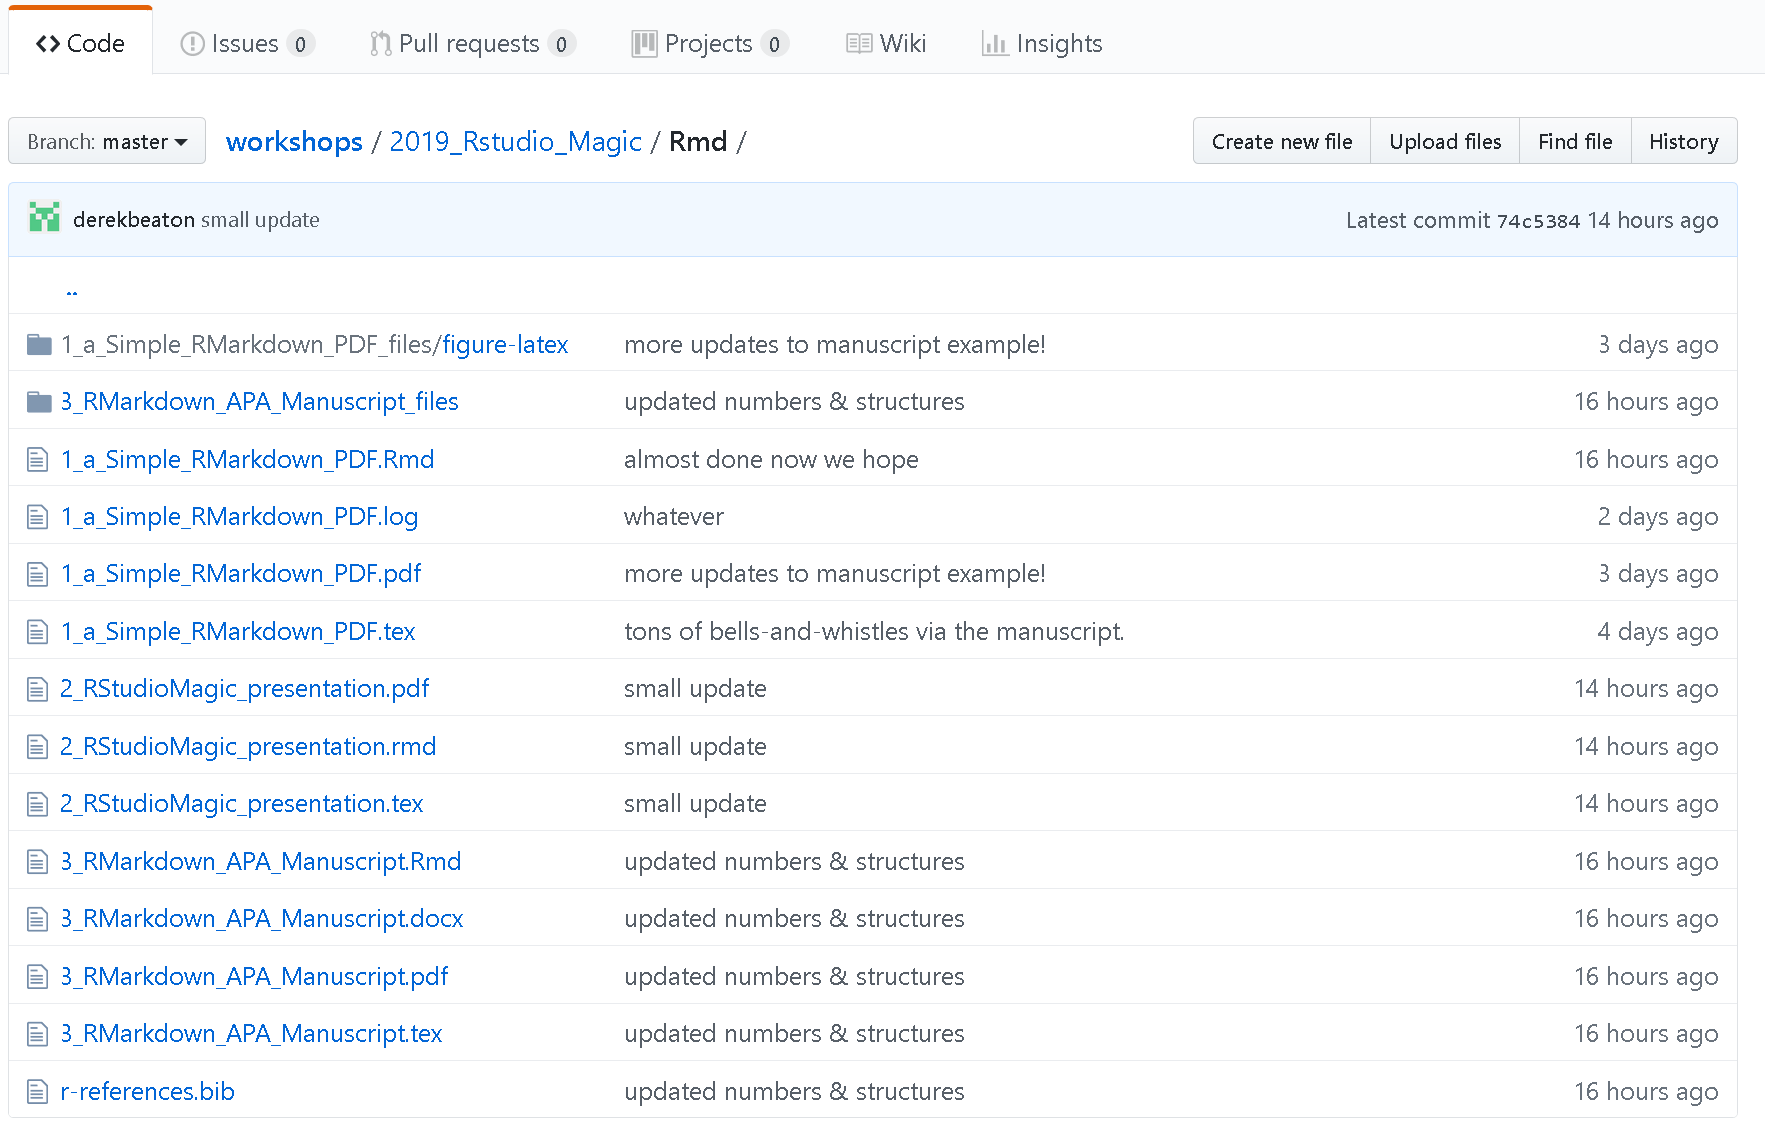
\includegraphics{../external/images/RMDfolder.PNG}

\end{frame}

\begin{frame}{RStudio Setup}
\protect\hypertarget{rstudio-setup-1}{}

\begin{itemize}
\tightlist
\item
  Download R and Rstudio
\item
  Strongly recommend Microsoft R (\url{https://mran.microsoft.com/open})

  \begin{itemize}
  \tightlist
  \item
    Comes with Intel MKL
  \end{itemize}
\item
  Plain R is fine (\url{https://cran.r-project.org/})

  \begin{itemize}
  \tightlist
  \item
    Can relink to faster libraries
  \end{itemize}
\item
  Download RStudio (\url{https://www.rstudio.com/})
\end{itemize}

\end{frame}

\begin{frame}[fragile]{Get the packages you need}
\protect\hypertarget{get-the-packages-you-need}{}

\begin{Shaded}
\begin{Highlighting}[]
\CommentTok{#to install from CRAN}
\KeywordTok{install.pacakges}\NormalTok{(}\StringTok{'devtools'}\NormalTok{, }\DataTypeTok{depenedencies =} \OtherTok{TRUE}\NormalTok{)}

\CommentTok{#to install from a git  (requires the devtools package)}
\NormalTok{dev.tools}\OperatorTok{::}\KeywordTok{install_github}\NormalTok{(Gibbsdavidl}\OperatorTok{/}\NormalTok{CatterPlots)}

\CommentTok{#to install from a file}
\KeywordTok{install.packages}\NormalTok{(}\StringTok{'/mypath/to/package/ADNIMERGE.tar.gz'}\NormalTok{, }
                 \DataTypeTok{type=}\StringTok{'source'}\NormalTok{, }\DataTypeTok{repos=}\OtherTok{NULL}\NormalTok{) }
\end{Highlighting}
\end{Shaded}

\end{frame}

\begin{frame}{Some transition?}
\protect\hypertarget{some-transition}{}

\end{frame}

\begin{frame}{R et al}
\protect\hypertarget{r-et-al}{}

\begin{itemize}
\tightlist
\item
  A bit of background, including idiosyncrasies and unique things about
  R

  \begin{itemize}
  \tightlist
  \item
    Especially packages \& three ways to install (somewhat covered
    above) CRAN, Locally, Git \& others (devtools)
  \item
    It's a functional language
  \item
    Data types Including data frames \& alts like tibbles
  \end{itemize}
\item
  Read/explore

  \begin{itemize}
  \tightlist
  \item
    explore .R scripts
  \end{itemize}
\item
  Clean/export

  \begin{itemize}
  \tightlist
  \item
    Show 0\_Create from PCA/MCA with Base, Tidyverse, Plyr (NOT dplyr),
    data.table
  \item
    Reimport?
  \item
    Analyze With MCA \& covstatis
  \end{itemize}
\end{itemize}

\end{frame}

\begin{frame}[fragile]{Read in and create your dataframe}
\protect\hypertarget{read-in-and-create-your-dataframe}{}

\begin{itemize}
\tightlist
\item
  ADNI Dataset adnimerge package

  \begin{itemize}
  \tightlist
  \item
    Reduce full dataset to only those participants (rows) and variables
    (columns) you're interested in
  \end{itemize}
\item
  Two methods to create your dataframe

  \begin{itemize}
  \tightlist
  \item
    using base R functions: \texttt{0\_create\_ADNI\_data\_base.R}
  \item
    Using tidyverse functions:
    \texttt{1\_create\_ADNI\_data\_tidyverse.R}
  \end{itemize}
\end{itemize}

\end{frame}

\begin{frame}{Screenshots}
\protect\hypertarget{screenshots}{}

Explanation

\end{frame}

\begin{frame}[fragile]{Exploring your data}
\protect\hypertarget{exploring-your-data}{}

\begin{itemize}
\tightlist
\item
  Many packages to help explore and describe your data:

  \begin{itemize}
  \tightlist
  \item
    summarytools: \texttt{2\_explore\_summarytools.R}
  \item
    inspectdf: \texttt{3\_explore\_inspectdf.R}
  \item
    DataExplorer: \texttt{4\_explore\_DataExplorer\_one\_liner.R}
  \end{itemize}
\end{itemize}

\end{frame}

\begin{frame}{Code w/ eval=F}
\protect\hypertarget{code-w-evalf}{}

\end{frame}

\begin{frame}{Hard Break}
\protect\hypertarget{hard-break}{}

\begin{itemize}
\tightlist
\item
  DataExplorer is dangerous
\item
  Blind analyses can be \emph{criminal}

  \begin{itemize}
  \tightlist
  \item
    de Leeuw paper quote
  \item
    DEREK RANTS, PER USUAL.
  \end{itemize}
\end{itemize}

\end{frame}

\begin{frame}[fragile]{Analyze you data}
\protect\hypertarget{analyze-you-data}{}

\begin{itemize}
\tightlist
\item
  Linear models: \texttt{5\_linear\_model.R}
\end{itemize}

\end{frame}

\begin{frame}{Screenshots / Code w/ eval=F}
\protect\hypertarget{screenshots-code-w-evalf}{}

\end{frame}

\begin{frame}[fragile]{Get experimental}
\protect\hypertarget{get-experimental}{}

\begin{itemize}
\tightlist
\item
  Explain motivation, not method
\item
  covSTATIS: \texttt{6\_covstatis\_example.R}
\end{itemize}

\end{frame}

\hypertarget{part-3-rmarkdown}{%
\section{Part 3: RMarkdown}\label{part-3-rmarkdown}}

\begin{frame}{RMarkdown}
\protect\hypertarget{rmarkdown}{}

\begin{itemize}
\tightlist
\item
  What it is /why to use it
\item
  A short deviation for LaTeX, and new helpers: kable \& kableExtra

  \begin{itemize}
  \tightlist
  \item
    A taxonomy and how to approach this \emph{Tying it all together
    through here 1: simple RMD }Plot-based visuals

    \begin{itemize}
    \tightlist
    \item
      Base, gt, ggplot, grobTable()/grid/gridExtra
    \item
      2: Slides (these ones here)
    \item
      3: Manuscripts!!
    \end{itemize}
  \end{itemize}
\item
  Reporting/presentin
\end{itemize}

\end{frame}

\begin{frame}[fragile]{RMarkdown Don(u)'ts}
\protect\hypertarget{rmarkdown-donuts}{}

\begin{itemize}
\tightlist
\item
  Don't hardcode values
\item
  Don't hardcode absolute file paths
\item
  Don't do complicated database queries
\item
  Don't litter

  \begin{itemize}
  \tightlist
  \item
    avoid \texttt{eval=FALSE}
  \item
    reduce repeated code by making functions
  \end{itemize}
\item
  Don't load unneccesary libraries
\item
  More at:
  \url{https://emilyriederer.netlify.com/post/rmarkdown-driven-development/}
\end{itemize}

\end{frame}

\hypertarget{part-4-advanced-r}{%
\section{Part 4: Advanced R}\label{part-4-advanced-r}}

\begin{frame}{Some advanced/other things we're not covering}
\protect\hypertarget{some-advancedother-things-were-not-covering}{}

\begin{itemize}
\tightlist
\item
  package development
\item
  Shiny
\item
  SQL
\item
  C/C++
\item
  R2D3
\end{itemize}

\end{frame}

\begin{frame}{A few of our favorite things}
\protect\hypertarget{a-few-of-our-favorite-things}{}

\begin{itemize}
\tightlist
\item
  Fun R do-dads
\end{itemize}

\end{frame}

\begin{frame}[fragile]{CatterPlot for feline based graphics:}
\protect\hypertarget{catterplot-for-feline-based-graphics}{}

\begin{itemize}
\tightlist
\item
  \url{https://github.com/Gibbsdavidl/CatterPlots}
\end{itemize}

\texttt{dev.tools::install\_github(Gibbsdavidl/CatterPlots)}

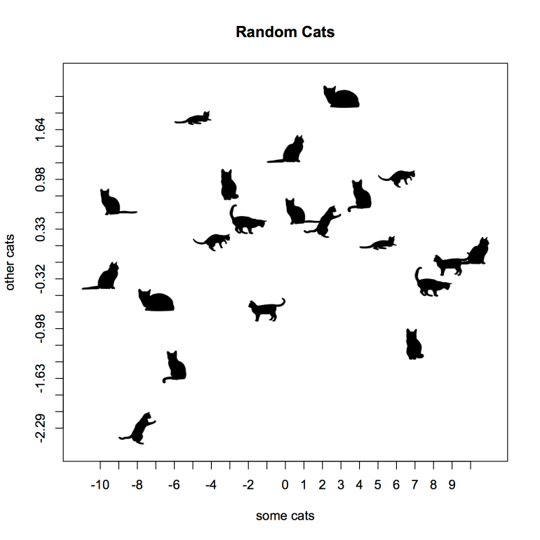
\includegraphics[width=0.6\textwidth,height=\textheight]{../external/images/funR_1_catterplotter.png}

\end{frame}

\begin{frame}[fragile]{What's a pirate's favorite programming language?}
\protect\hypertarget{whats-a-pirates-favorite-programming-language}{}

\begin{itemize}
\tightlist
\item
  \url{https://cran.r-project.org/web/packages/yarrr/vignettes/pirateplot.html}
\end{itemize}

\texttt{install.packages(\textquotesingle{}yarrr\textquotesingle{})}

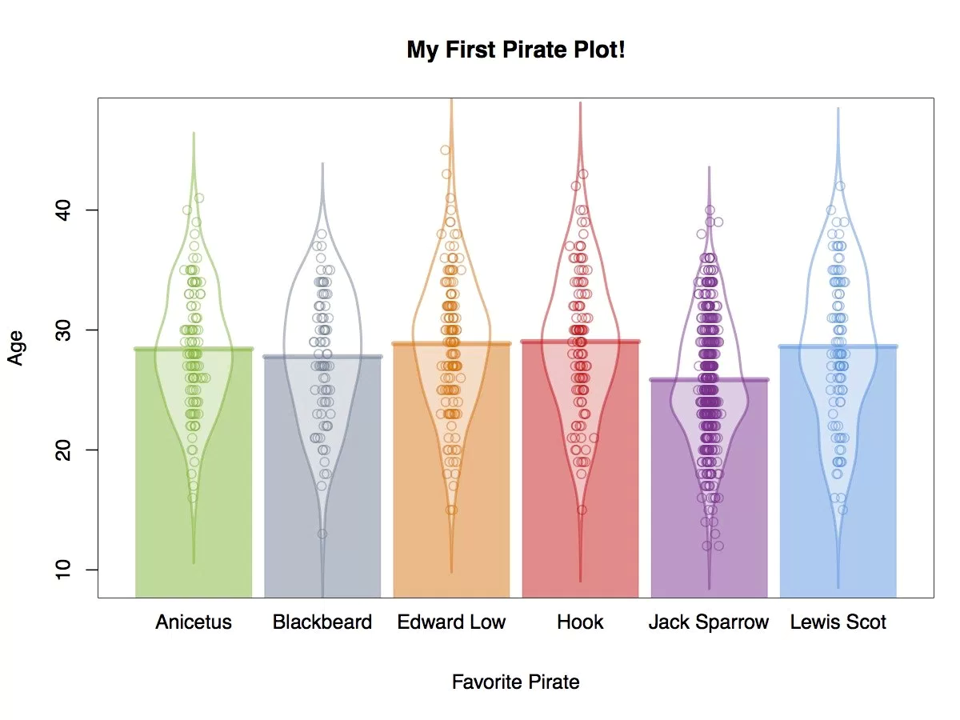
\includegraphics[width=0.75\textwidth,height=\textheight]{../external/images/funR_2_pirate.png}

\end{frame}

\begin{frame}[fragile]{Color palettes to fit your \textsubscript{mood}}
\protect\hypertarget{color-palettes-to-fit-your-mood}{}

\begin{itemize}
\tightlist
\item
  \url{https://github.com/karthik/wesanderson}
\end{itemize}

\texttt{dev.tools::install\_github(karthik/wesanderson)}

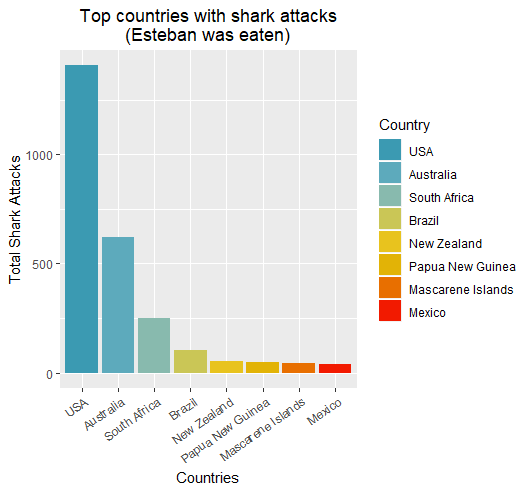
\includegraphics{../external/images/funR_3_wes_anderson.png}

\end{frame}

\begin{frame}[fragile]{Mapping your Strava routes}
\protect\hypertarget{mapping-your-strava-routes}{}

\begin{itemize}
\tightlist
\item
  \url{https://www.r-bloggers.com/strava-rides-map-in-r/}
\item
  ALSO \url{https://marcusvolz.com/?p=4068}

  \begin{itemize}
  \tightlist
  \item
    \texttt{dev.tools::install\_github(marcusvolz/strava)}
  \end{itemize}
\end{itemize}

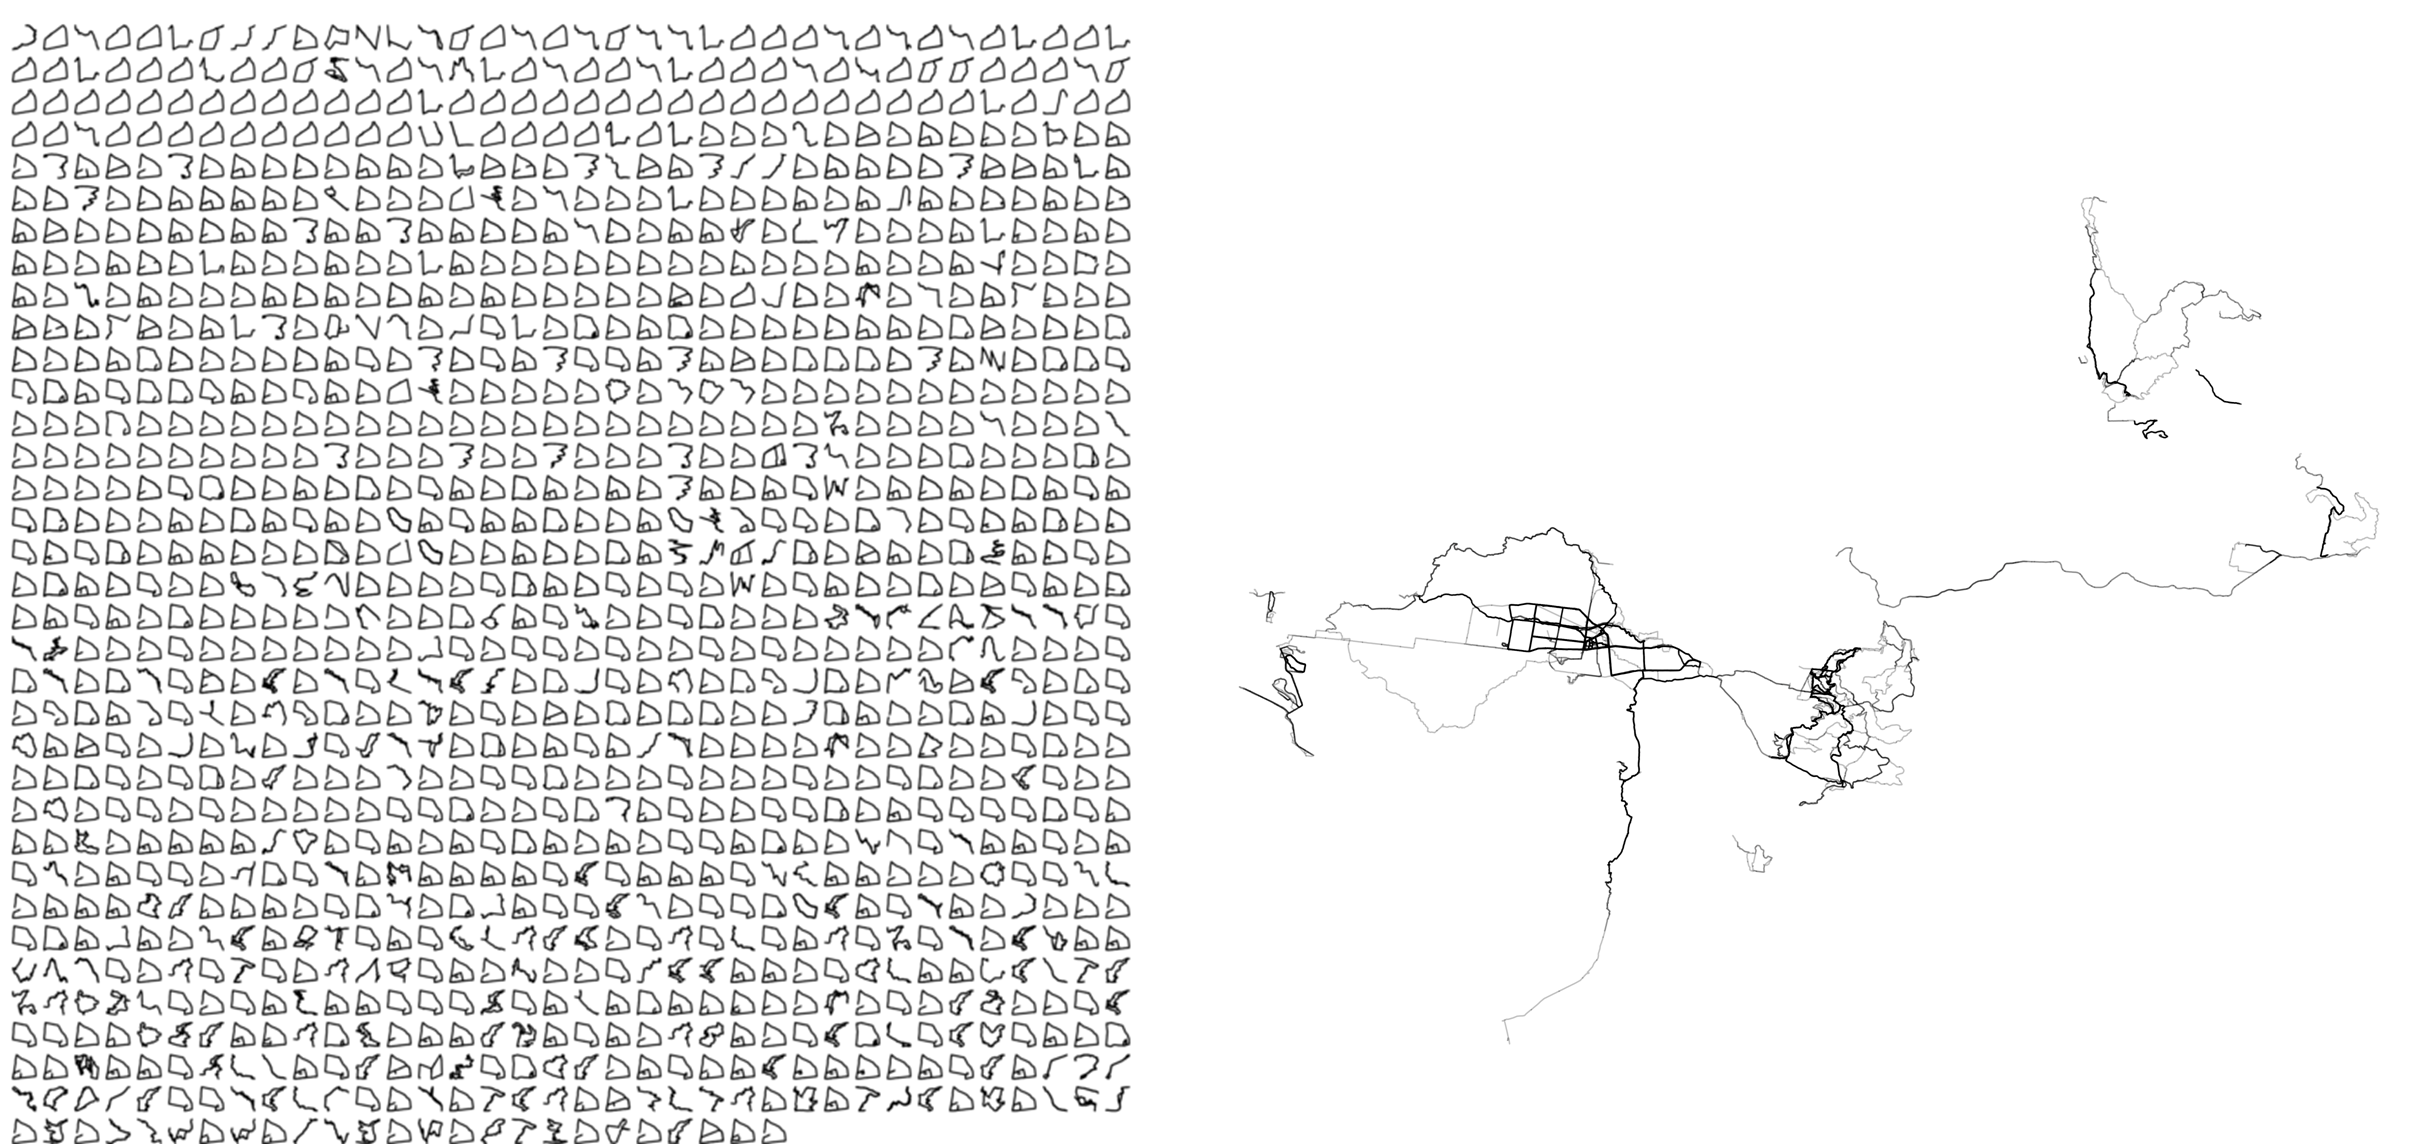
\includegraphics{../external/images/funR_4_strava_combo.png}

\end{frame}

\begin{frame}{Make aRt!}
\protect\hypertarget{make-art}{}

\begin{itemize}
\tightlist
\item
  R Graph Gallery

  \begin{itemize}
  \tightlist
  \item
    \url{http://www.r-graph-gallery.com/}
  \end{itemize}
\item
  Rtist: Gaston Sanchez

  \begin{itemize}
  \tightlist
  \item
    \url{http://gastonsanchez.com/Rtist/}
  \end{itemize}
\end{itemize}

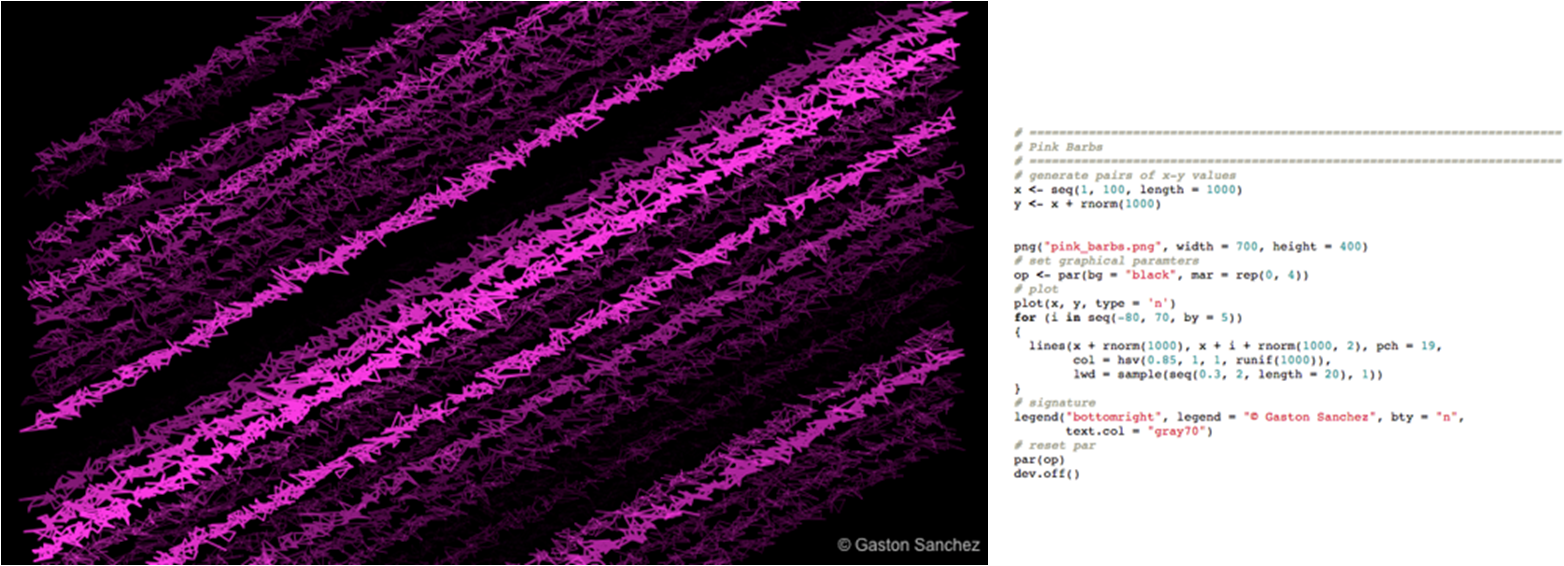
\includegraphics{../external/images/funR_5_aRt_pink_combo.png}

\end{frame}

\end{document}
